\chapter{Environment Exploration}%
\label{CH:EXPLORATION}

%----------------------------------------------------------------------------------------
\section{The Framework}%
\label{SEC:EXPLORATION-FRAMEWORK}
The ability to autonomously plan and execute informative trajectories in previously unknown, or partially known,
environments is a fundamental requirement for mobile robots. As a matter of fact, they started to be employed
in a huge number of different applications which require the ability to efficiently collect new information
about the surroundings, such as surface inspection, object search, weed recognition, search and rescue missions, and others.
The problem of Informative Path Planning (IPP), jointly with the problem of environment exploration, has been extensively
studied in literature and a wide variety of approaches have been proposed so far. The majority of recent works had
focused on novel hybrid approaches leveraging the interplay between the concepts of \emph{local} and \emph{global}
exploration~\cite{selin2019efficient,schmid2020efficient}. In particular, the major issue behind such works is related
to how efficiently combine the two local and global exploration steps, and how to plan highly informative global
paths out of the current environment information. A limited number of papers focused on improving the local exploration
step~\cite{selin2019efficient}. On the other hand, the necessity to push the autonomous platform always toward unknown
frontiers limited the research of solutions where the environment is a priori known, or partially known, and the agent
should perform patrolling-like operations~\cite{dang2018autonomous}. In this chapter, we present two novel approaches
aiming, in the first stage, to push the current state-of-the-art toward more smooth and resilient solutions for local
exploration in cluttered and possibly varying environments, and, in the second stage, to adapt global exploration tools
to the problem of fast environment patrolling and object search.

\subsection{Related Works}%
\label{SEC:EXPLORATION-RELATED-WORKS}
Although the number of solutions presented in the literature is quite variegated, the majority of them can be classified as
\emph{frontier-based} or \emph{sampling-based} methods. The former class was pioneered in~\cite{yamauchi1997frontier} and
later more comprehensively developed in~\cite{julia2012comparison}. The key idea is to guide the agent toward the borders
between free and unmapped space (aka frontiers), since these points may represent those with higher potential information gain.
Exploration is then carried out by extracting the map frontiers and by navigating through them sequentially.
Several works propose to extend it by adding constraints to ensure low localization errors~\cite{stachniss2005information}.
The basic frontier-based approach has been also extended to high-speed flight for fast exploration in~\cite{cieslewski2017rapid}.
In this case, the authors propose to extract frontiers only inside the current Field-Of-View (FoV) and select the one leading
to the minimal change in velocity. In recent years, other works focused on rapid exploration~\cite{zhou2021fuel}, by planning
global coverage paths and optimising them with respect to the robot dynamics, and on the reformulation of the frontier information
gain as a differentiable function~\cite{deng2020robotic}, allowing paths to be optimised with gradient information. On the other hand,
\emph{sampling-based} methods typically sample random viewpoints to explore the space in a Next-Best-View (NBV)
fashion~\cite{connolly1985determination, maver1993occlusions}. Much of the work in this domain can be traced back
to~\cite{gonzalez2002navigation}, where the NBV problem has been moved for the first time from the computer graphic field to the
robotic domain, with the introduction of the notion of reconstruction gain. The concept of NBV exploration has been afterward extended
by~\cite{bircher2016receding}, where the building of a Rapidly-Exploring Random Tree (RRT) allows one to weigh both the amount of
information gained at the viewpoints and during the agent motion to reach each viewpoint. Unlike frontier-based methods, which
are difficult to adapt to other tasks, the sampling-based ones have the advantage to allow any kind of gain formulation.
Thanks to that, the original NBV algorithm was extended to consider the uncertainty of localisation~\cite{papachristos2017uncertainty, tovar2006planning}
and the visual importance of different objects~\cite{dang2018visual}. On the other hand, sampling-based methods suffer from stacking
in local minima, leading to a premature ending of the exploration procedure in unlucky scenarios. For this reason, the recent trend is
to merge the two frontiers and sampling-based approaches in a local-global exploration fashion. The pioneer of this idea
was~\cite{charrow2015information}, which makes use of a frontier method to detect global goals and supplements these with motion primitives
for local exploration. More recent approaches, instead, leverage the capabilities of sampling-based methods and employ additional planning
stages to escape from local minima~\cite{selin2019efficient,dang2019graph}. Other approaches focus on memorising previously visited places
and sampled information under the format of roadmaps~\cite{witting2018history, xu2021autonomous}. Similarly, the work presented
in~\cite{schmid2020efficient} continuously maintains and expands a single RRT of candidate paths. Although the literature has seen some
impressive works in the field of NBV, there are very few works concentrating on fast exploration. Even if previous solutions are able to
quickly plan global coverage paths~\cite{schmid2020efficient, xu2021autonomous, kompis2021informed}, the problem of efficient trajectory
planning is rarely addressed. Both under the perspective of local exploration and the patrolling, or object finding, problem.

\subsection{Problem Definition}%
\label{SEC:EXPLORATION-PROBLEM-DEFINITION}
The problem addressed in this chapter consists of exploring, as fast as possible, a bounded 3D volume $\V \subset \R^3$.
Each point $ \xx = \lp x, y, z \rp \in \V$ of this space can take only two values, i.e. \emph{free} or \emph{occupied},
and  the problem of exploration ideally consists of clustering the volume $\V$ in the free
$\V_{\text{free}} = \{ \xx \in \V \mid \Gamma(\xx) = \text{free} \}$ or occupied
$\V_{\text{occ}} = \{ \xx \in \V \mid \Gamma(\xx) = \text{occ} \}$ volumes, with a mapping function
$\Gamma(\xx): \V \mapsto \left\{ \text{free}, \text{occ} \right\}$.
Since this operation is subjected to the agent constraints and its sensing capabilities, it may happen that some map point
cannot be observed by construction. These points will remain unmapped and, for this reason, we introduce a further set
$\V_{\text{res}}$ collecting the residual points that cannot be observed. Thus, the exploration will be considered complete
when $\V_{\text{free}} \cup \V_{\text{occ}} = \V \setminus \V_{\text{res}}$. Due to the nature of the problem, it has to be
solved in real-time by planning suitable safe trajectories through the free space which is not known a priori.

%----------------------------------------------------------------------------------------
\section{Large-Scale Environments Exploration}%
\label{SEC:EXPLORATION-LARGE-SCALE}
In this section, we propose a novel solution to the aforementioned exploration problem (\secref{SEC:EXPLORATION-PROBLEM-DEFINITION})
in a setting where timing is the major issue during the task of completely unknown environment exploration. The basic idea behind the
proposed solution is that efficient local procedures allow for a very high speed up in the overall task. Although the global-local
paradigm is fundamental to ensure consistency and completeness of the exploration procedure, it is not the key to compute efficient 
exploration paths, due to the fact that the switching between local and global may lead to a waste of time, requiring the agent 
to change direction very frequently. On the other hand, optimising local trajectories with respect to the agent capabilities and
the locally gathered information of the environment under exploration may lead to faster motions, low energy consumption, and lower
waste of time. This is especially true when dealing with Unmanned Aerial Vehicles (UAVs), whose high maneuverability motivates solutions
able to stress the quadrotor to fully exploit both its computational and dynamical capabilities.
Similarly to~\cite{selin2019efficient} and~\cite{bircher2016receding}, the core of the proposed solution consists of an RRT-inspired~\cite{lavalle1998rapidly}
sampling-based exploration algorithm that aims to directly plan highly informative feasible trajectories in known space, leading to an
optimal local exploration procedure. The obtained tree is executed one node at a time, in a receding-horizon fashion.
Unlike previous works, our algorithm employs a B\acuteacc ezier curve parameterisation to grow and maintain a tree of possible trajectory
segments. The proposed approach weights both potential information gain and trajectory cost during the selection of the next goal.
Moreover, the planned trajectory does not constrain the end velocity to zero, thus the exploration can be performed quickly
by avoiding ``stop-and-go'' like behaviors. Motivated by the promising results obtained using hybrid approaches~\cite{selin2019efficient},
we allow adaptability of the proposed solution by letting the tree be easily extended with global exploration routines.
In particular, we implemented efficient rewiring procedures in order to keep in memory and continuously refine the same tree, following
the ideas of roadmaps memorisation~\cite{xu2021autonomous} and continuous tree expansion~\cite{schmid2020efficient}.
We show that the combination of the planning of both path and the associated timing law leads to a solution outperforming the state-of-the-art approaches
in this field, which usually plans point-to-point trajectories requiring stopping the robot at each exploration step.

\subsection{B\acuteacc ezier Trajectory Parameterisation}%
\label{SEC:EXPLORATION-TRAJECTORY-PARAMETERISATION}
In this framework, instead of using traditional polynomial functions, we adopt the Bernstein polynomial basis and define trajectories as
piecewise B\acuteacc ezier curves. A B\acuteacc ezier curve is completely defined by its degree $\order$ and a set of $\cpnumber = \order+1$
control points $\CP = \lps \bs{\cpoint}_0 \cdots \bs{\cpoint}_{\order} \rps$, with $\bs{\cpoint}_i \in \R$. The curve can be evaluated, for any
$ \splinevar \in [0, 1]$, as
\begin{equation}
	\label{EQ:BEZIER-SIMPLE}
	\bs{\spline} \lp \splinevar \rp = \sum_{i=0}^{\order} \basis_i^{\order}\lp \splinevar \rp \bs{\cpoint}_i,
\end{equation}
where the basis functions $\basis_i^{\order} \lp \splinevar \rp$ are $\order$th degree
\emph{Bernstein basis polynomials}~\cite{farouki2012bernstein, biagiotti2008trajectory} of the form
\begin{equation*}
	\basis_i^{\order}\lp \splinevar \rp = \frac{\order!}{i!(\order - i)!} \splinevar^i {(1 - \splinevar)}^{\order - i}.
\end{equation*}
A gentle introduction to B\acuteacc ezier curves can be found in~\appref{SEC:SPLINES-APPENDIX}, to seek of clarence we report here the major
properties required to properly understand the subsequent analysis. The aforementioned polynomials enjoy a partition-of-unity property
(i.e. $\sum_{i=0}^{\order} \basis_i^{\order} \lp \splinevar \rp = 1$ for all $\splinevar$), by which the curve defined by~\eqqref{EQ:BEZIER-SIMPLE}
is constrained inside the convex hull generated by its control points $\CP$. Moreover, a $\order$-degree B\acuteacc ezier curve is always
$\order$ times differentiable and its derivatives preserve a B\acuteacc ezier structure of lower degree. In particular,
$\spline' \lp \splinevar \rp := d\spline/d\splinevar$ is a B\acuteacc ezier curve of order $\order-1$ whose control points $\CP'$ can be
evaluated as $\bs{\cpoint}'_i = \order \lp \bs{\cpoint}_{i+1} - \bs{\cpoint}_i \rp$ $\forall i = 0, \dots, \order-1.$ The overall quadrotor reference
trajectory can be expressed through the evolution of its \emph{flat outputs}~\cite{mellinger2011minimum}, as explained in~\secref{SEC:DIFFERENTIAL-FLATNESS},
$\flatoutput = {\lps \rr, \yaw \rps}\T$, where $\rr = {\lps x, y, z \rps}\T \in \R^3$ represents the coordinates of the
center of mass in the world coordinate system, while $\yaw \in \R$ is the yaw angle. Both the quantities $\rr$ and $\yaw$ are expressed as
$\segnumber$-segments piecewise B\acuteacc ezier curves of order $\order_{\rr}$ and $\order_{\yaw}$, respectively
\begin{equation*}
	\rr \lp t \rp=
	\begin{cases}
		\sum_{i=0}^{\order_{\rr}} \basis_i^{\order_{\rr}}(\clock_1) \rr^1_i & \hspace{-0.2cm} t \in [T_0, T_1],\\
		\sum_{i=0}^{\order_{\rr}} \basis_i^{\order_{\rr}}(\clock_2) \rr^2_i & \hspace{-0.2cm} t \in [T_1, T_2],\\
		\hspace{0.2cm} \vdots & \vdots \\
		\sum_{i=0}^{\order_{\rr}} \basis_i^{\order_{\rr}}(\clock_{\segnumber}) \rr^{\segnumber}_i & \hspace{-0.2cm} t \in [T_{\segnumber-1}, T_{\segnumber}],\\
	\end{cases}
\end{equation*}
\begin{equation*}
	\yaw \lp t \rp=
	\begin{cases}
		\sum_{i=0}^{\order_{\yaw}} \basis_i^{\order_{\yaw}}(\clock_1) \yaw^1_i & \hspace{-0.2cm} t \in [T_0, T_1],\\
		\sum_{i=0}^{\order_{\yaw}} \basis_i^{\order_{\yaw}}(\clock_2) \yaw^2_i & \hspace{-0.2cm} t \in [T_1, T_2],\\
		\hspace{0.2cm} \vdots & \vdots \\
		\sum_{i=0}^{\order_{\yaw}} \basis_i^{\order_{\yaw}}(\clock_{\segnumber}) \yaw^{\segnumber}_i & \hspace{-0.2cm} t \in [T_{\segnumber-1}, T_{\segnumber}],\\
	\end{cases}
\end{equation*}
with $\clock_i = \frac{t-T_{i-1}}{T_{i}-T_{i-1}}$. The quantities $\rr_i^j \in \R^3$ and $\yaw_i^j \in \R$ describe the $i^{th}$ control
point of the $j^{th}$ trajectory segment of $\rr(t)$ and $\yaw(t)$ respectively, while $T_{j-1}$ and $ T_j$ are the start and end time of
the $j^{th}$ trajectory segment. Note that the introduced time scaling does not affect the spatial path described by the B\acuteacc ezier
curve, but strongly affects its derivatives as 
\begin{align*}
	{\rr'}^j_i & = \frac{\order_{\rr}(\rr^j_{i+1}-\rr^j_i)}{T_{j-1}-T_j} \hspace{0.2cm} \forall i=0,\dots,\order_{\rr}-1 , \\
	{\yaw'}^j_i & = \frac{\order_{\yaw}(\yaw^j_{i+1}-\yaw^j_i)}{T_{j-1}-T_j} \hspace{0.2cm} \forall i=0,\dots,\order_{\yaw}-1 .
\end{align*}
\begin{figure}[!t]
	\begin{minipage}{.45\linewidth}
		\centering
		\subfloat[]{%
			\label{FIG:EXPLORATION-BEZIER-CURVE-A}%
			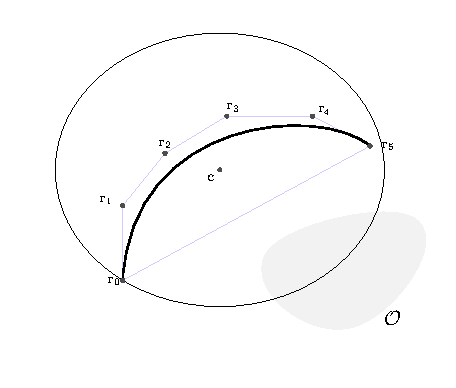
\includegraphics[scale=.85]{Figs/Chapter4/bezier_conservative.pdf}}
	\end{minipage}
	\begin{minipage}{.45\linewidth}
		\centering
		\subfloat[]{%
			\label{FIG:EXPLORATION-BEZIER-CURVE-B}%
			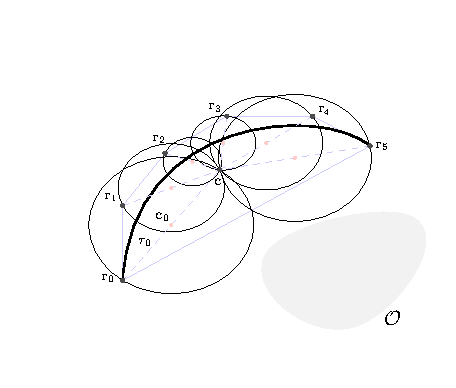
\includegraphics[scale=.85]{Figs/Chapter4/bezier_envelope.pdf}}
	\end{minipage}
	\caption{Representation of a fifth-degree B\acuteacc ezier curve with
	(a) the classical sphere used for collision checking~\cite{tang2020real}
	(b) the proposed multiple spheres envelope.
	The $\mathcal{O}$ shaded gray area represents a generic obstacle.}\label{fig:BEZIER-CURVE}
\end{figure}
The \emph{convex hull containment} property is a powerful tool to verify both the trajectory feasibility in terms of dynamic constraints,
such as velocity or acceleration bounds, and to check for collisions. \figref{FIG:EXPLORATION-BEZIER-CURVE-A} reports the classical
condition used for collision checking with B\acuteacc ezier curves~\cite{tang2020real}, where the overall curve is constrained inside a
\emph{safe} sphere. The aforementioned approach often results in being too conservative, as a matter of fact the considered sphere
is far to be tight over the convex hull, and thus over the curve itself. For this reason we formulate a new proposition that represents
a less conservative tool to verify collision (see \figref{FIG:EXPLORATION-BEZIER-CURVE-B}).
\begin{proposition}%
	\label{PROPOSITION:EXPLORATION-ENVELOPE-CONTAINMENT}
	Let $\rr \lp \splinevar \rp$ be a B\acuteacc ezier curve of order $\order$, with control points $\CP= \lps \rr_0, \dots, \rr_{\order} \rps$.
	Moreover, let $\ri_i \in \R$  and $\cc_i \in \R^3$ with $i=0, \dots, \order$ be respectively the radii and centre of $\order$ spheres
	($\mathcal{C}_0 \dots \mathcal{C}_{\order}$), defined as:
	\begin{equation*}
		\begin{split}
			\cc_i & = (\rr_i + \cc)/2, \\
			\ri_i & = \norm{\rr_i - \cc_i},
		\end{split}
	\end{equation*}
	with $\cc$ be the centre of the convex hull generated by $\CP$, i.e. $\cc = \sum_{i=0}^{\order} \rr_i/\order$.
	Then the curve $\rr \lp \splinevar \rp$ is entirely contained inside the spheres envelope, namely
	\begin{equation*}
		\rr \lp \splinevar \rp \in \bigcup_{i=1}^{\order} \mathcal{C}_i \hspace{0.5cm} \forall \splinevar \in [0,1].
	\end{equation*}
\end{proposition}
\begin{proof}
    The proof follows from the fact that $\cc$ belongs to the convex hull and that the spheres envelope composed by
	$\mathcal{C}_i$ and $\mathcal{C}_{i+1}$ always contains the convex hull edge $\overline{\rr_i\rr_{i+1}}$.
	The first statement is true by construction, since $\cc$ is a linear combination of $\rr_i$, while the second one
	follows from the triangle inequality
	\begin{equation*}
		\norm{\rr_i - \rr_{i+1}} \le \norm{\rr_i - \cc} + \norm{\rr_{i+1} - \cc}. \qedhere
	\end{equation*} 
\end{proof}
\propref{PROPOSITION:EXPLORATION-ENVELOPE-CONTAINMENT} states that the convex hull containment property can be reformulated taking
into account a set of $\order$ spheres. Since this set of spheres results to be tighter around the curve with respect to a single big
safe ball, the use of this proposition in formulating a new collision condition results in a less conservative approach.
The following proposition states the sufficient condition for non-collision as a corollary of~\propref{PROPOSITION:EXPLORATION-ENVELOPE-CONTAINMENT}.
\begin{proposition}%
	\label{PROPOSITION:EXPLORATION-COLLISION-FREE}
	Let $\rr \lp \splinevar \rp$ be a B\acuteacc ezier curve of order $\order$, with control points $\CP= \lps \rr_0, \dots, \rr_{\order} \rps$.
	Moreover, let $\cc_i$ and $\ri_i$ with $i=0,\dots,\order$ be the centre and radii of $\order$ spheres defined as
	in~\propref{PROPOSITION:EXPLORATION-ENVELOPE-CONTAINMENT}. The curve $\rr \lp \splinevar \rp$ is said to be collision-free,
	with a safety bound of $d^{\text{safe}} \in \R_{+}$, if the condition
	\begin{equation*}
		\ri_i - d^{\text{obs}}_{\cc_i} - d^{\text{safe}} > 0 \hspace*{0.5cm} \forall i = 0, \dots, \order
	\end{equation*}
	holds, where $d^{\text{obs}}_{\cc_i}$ represents the Euclidean distance of $\cc_i$ from the closest obstacle.
\end{proposition}
From now on, we use fifth-order B\acuteacc ezier curves to represent the quadrotor position ($\order_{\rr} = 5$),
while the yaw trajectory is parameterised using third-order B\acuteacc ezier curves ($\order_{\yaw} = 3$).

\subsection{Tree Structure}%
\label{SEC:EXPLORATION-TREE-STRUCTURE}
The proposed algorithm works by growing and maintaining, at each iteration, a tree $\tree = \lp \nodes, \edges \rp$ of possible trajectories.
Such tree consists of a set of nodes $\nodes = \{\node_1, \dots, \node_{\dd{\node}}\}$ and a set of edges
$\edges = \{\edge_i, \dots , \edge_{\dd{\edge}}\}$. Each node $\node_i$ is completely defined by the following five quantities
\begin{equation*}
	\node_i = \left\{ g_i, c_i, \delta_i, \CP^{\rr}_i, \CP^{\yaw}_i \right\}
\end{equation*}
where $g_i = g \lp \node_i \rp$ represents the amount of information gained if that node is executed, and $c_i = c \lp \node_i \rp$
is the cost associated to the node execution. $\CP^{\rr}_i$ and $\CP^{\yaw}_i$ are the two sets of control points defining the
trajectories $\rr_i(t)$ and $\yaw_i(t)$, while $\delta_i$ is the execution time. Two nodes $\node_{i-1}$ and $\node_{i}$ are connected
by an edge $\edge_{i-1}$ only if the first $(\order_{\rr/\yaw}+1)/2$ control points of the latter node satisfy some continuity criterion with
the last $(\order_{\rr/\yaw}+1)/2$ control points of the former one. This constraint is required to ensure continuity among all trajectory
segments of the tree. In particular, since $\order_{\rr} = 5$ and $\order_{\yaw} = 3$, we enforce continuity up to the third derivative along
$\rr(t)$ and continuity up to the second derivative along $\yaw(t)$, namely
\begin{align}
	\label{EQ:EXPLORATION-FIRST-COND}
	&\rr^{i}_0  = \rr^{i-1}_5,\\
	\label{EQ:EXPLORATION-SECOND-COND}
	&\frac{1}{\delta_{i}}(\rr^{i}_1 - \rr^{i}_0)  = \frac{1}{\delta_{i-1}}(\rr^{i-1}_5 - \rr^{i-1}_4),\\
	\label{EQ:EXPLORATION-THIRD-COND}
	&\frac{1}{\delta_{i}^2}(\rr^{i}_2 - 2\rr^{i}_1 + \rr^{i}_0)  = \frac{1}{\delta_{i-1}^2}(\rr^{i-1}_5 - 2\rr^{i-1}_4 + \rr^{i-1}_3),\\
	\label{EQ:EXPLORATION-FOURTH-COND}
	&\yaw^{i}_0  = \yaw^{i-1}_3,\\
	\label{EQ:EXPLORATION-FIFTH-COND}
	&\frac{1}{\delta_{i}}(\yaw^{i}_1 - \yaw^{i}_0)  = \frac{1}{\delta_{i-1}}(\yaw^{i-1}_3 - \yaw^{i-1}_2).
\end{align}
The aim is to plan sub-optimal trajectories by maximising a user-specified utility function $\loss \lp \RR \lp \node_i \rp \rp$,
with $\RR \lp \node_i \rp$ be the sequence of nodes connecting $\node_i$ to the tree root, which properly combines gains and costs
of all nodes in $\RR \lp \node_i \rp$. In this context, the tree root is defined as the tree node which is about to be executed by the
flying agent. It results that the agent behavior strongly depends on the choice of functions $g \lp \node_i \rp$, $c \lp \node_i \rp$
and $\loss \lp \RR \lp \node_i \rp \rp$. The proposed algorithm is agnostic with respect to these functions. Therefore, the user can specify
any formulation of them by ensuring that the following criteria are satisfied~\cite{schmid2020efficient}:
\begin{enumerate}
	\item $g \lp \node_i \rp$ should be a function that depends on the trajectory end position only ($g \lp \rr^i_5, \yaw^i_3 \rp$),
	\item all node gains should be mutually independent,
	\item $c \lp \node_i \rp$ is required to be an intrinsic property of the trajectory ($c\lp\CP^{\rr}_i, \CP^{\yaw}_i, \delta_i\rp$).
\end{enumerate}

\subsection{Tree Update}%
\label{SEC:EXPLORATION-TREE-UPDATE}
The tree, initially composed by just one root node, is iteratively expanded by randomly sampling viewpoints inside a sphere centred on
the current \emph{best node} ($\node_{\text{best}}$), namely the one among all tree nodes that maximise the utility function $\loss(\cdot)$.
In particular, the sphere is centred exactly on the last control point of $\CP^{\rr}_{\text{best}}$, i.e. $\rr^{\text{best}}_5$, while
its radius ($r_{\text{sp}}$) is a user chosen value defined as a parameter for the algorithm. The sampled viewpoint is retained only if
it belongs to a known and free part of the environment under exploration and, at the same time, it is far enough from the mapped obstacles.
Such viewpoint is considered as the last control point of the next trajectory segment ($\rr^{i}_5$). Moreover, due to
Condition~\eqref{EQ:EXPLORATION-FIRST-COND}, also the control point $\rr^{i}_0$ is already defined to ensure position continuity.
As regards the heading trajectory, the first control point ($\yaw^i_0$) is established through Condition~\eqref{EQ:EXPLORATION-FOURTH-COND},
while the last one ($\yaw^i_3$) is chosen as the value that maximise the potential information gain $g(\rr_5^i, \yaw)$, namely
\begin{equation*}
	\yaw_i^3 = \arg \max_{\yaw} \ g(\rr_5^i, \yaw),
\end{equation*}
in a similar way as done in~\cite{selin2019efficient}. The choice of the remaining points ($\CP^{\rr}_i\lps 1:4 \rps$,
$\CP^{\yaw}_i \lps 1:2 \rps$) and the trajectory duration ($\delta_i$) is performed concurrently. In particular, the interval of
admissible trajectory duration $\Delta = [\delta_{\text{min}}, \delta_{\text{max}}]$ is uniformly discretised as
\begin{equation*}
	\Delta_{\text{d}} = \left\{ \delta_{\text{min}},\  \delta_{\text{min}} + \Delta_{\delta}, \  \delta_{\text{min}} + 2\Delta_{\delta},\  \dots, \ \delta_{\text{max}} \right\},
\end{equation*}
with $\Delta_{\delta} = \frac{\delta_{\text{max}} - \delta_{\text{min}}}{r}$, leading to $r+1$ possible time intervals.
For any $\delta \in \Delta_{\text{d}}$, the control points $\rr^{i}_1$ and $\rr^{i}_2$ are computed exploiting Condition~\eqref{EQ:EXPLORATION-SECOND-COND}
and Condition~\eqref{EQ:EXPLORATION-THIRD-COND}. If the obtained points do not satisfy~\propref{PROPOSITION:EXPLORATION-COLLISION-FREE}
the current $\delta$ is discarded, otherwise also the points $\rr^{i}_3$ and $\rr^{i}_4$, as well as $\yaw^i_1$
(Condition~\eqref{EQ:EXPLORATION-FIFTH-COND}) and $\yaw^i_2$ are computed.  Note that the quantities $\rr^{i}_3$, $\rr^{i}_4$ and
$\yaw^i_2$ are not constrained by any conditions~\eqref{EQ:EXPLORATION-FIRST-COND}--\eqref{EQ:EXPLORATION-FIFTH-COND}, thus these points
are computed by optimising the induced cost $c(\CP_i^{\rr}, \CP_i^{\yaw}, \delta_i)$. In the same way as before, if the computed points
violate~\propref{PROPOSITION:EXPLORATION-COLLISION-FREE}, or the induced velocity or acceleration exceed the dynamic bounds,
the current $\delta$ is discarded. Once all $\delta \in \Delta_{\text{d}}$ have been considered, the one leading to the optimal value
of $c_i$ is selected with the corresponding computed control points and the node is added to the tree.
The tree growth continues until it became impossible to find a new node with higher information gain $g(\cdot)$ and the number
of sampled nodes goes beyond a given threshold ($n_{\text{max}}$). Once the tree expansion is terminated, the branch leading to
the best node is extracted and only the first node of such branch ($\node_\text{opt}$) is executed.

It may happen that the tree growth procedure takes too much time, or it may result impossible to find a
valid candidate as next trajectory segment. In order to handle these issues, at each iteration two trajectory segments are computed.
The first one corresponds to the execution of the best branch, while the second one is a \emph{safe} trajectory,
linked via Constraints~\eqref{EQ:EXPLORATION-FIRST-COND}--\eqref{EQ:EXPLORATION-FIFTH-COND} to the first committed segment.
The \emph{safe} trajectory constrains the final velocity to be zero, as well as the final acceleration, and it is executed every time
the algorithm fails in planning a new node.
\begin{figure}[!t]
	\centering
	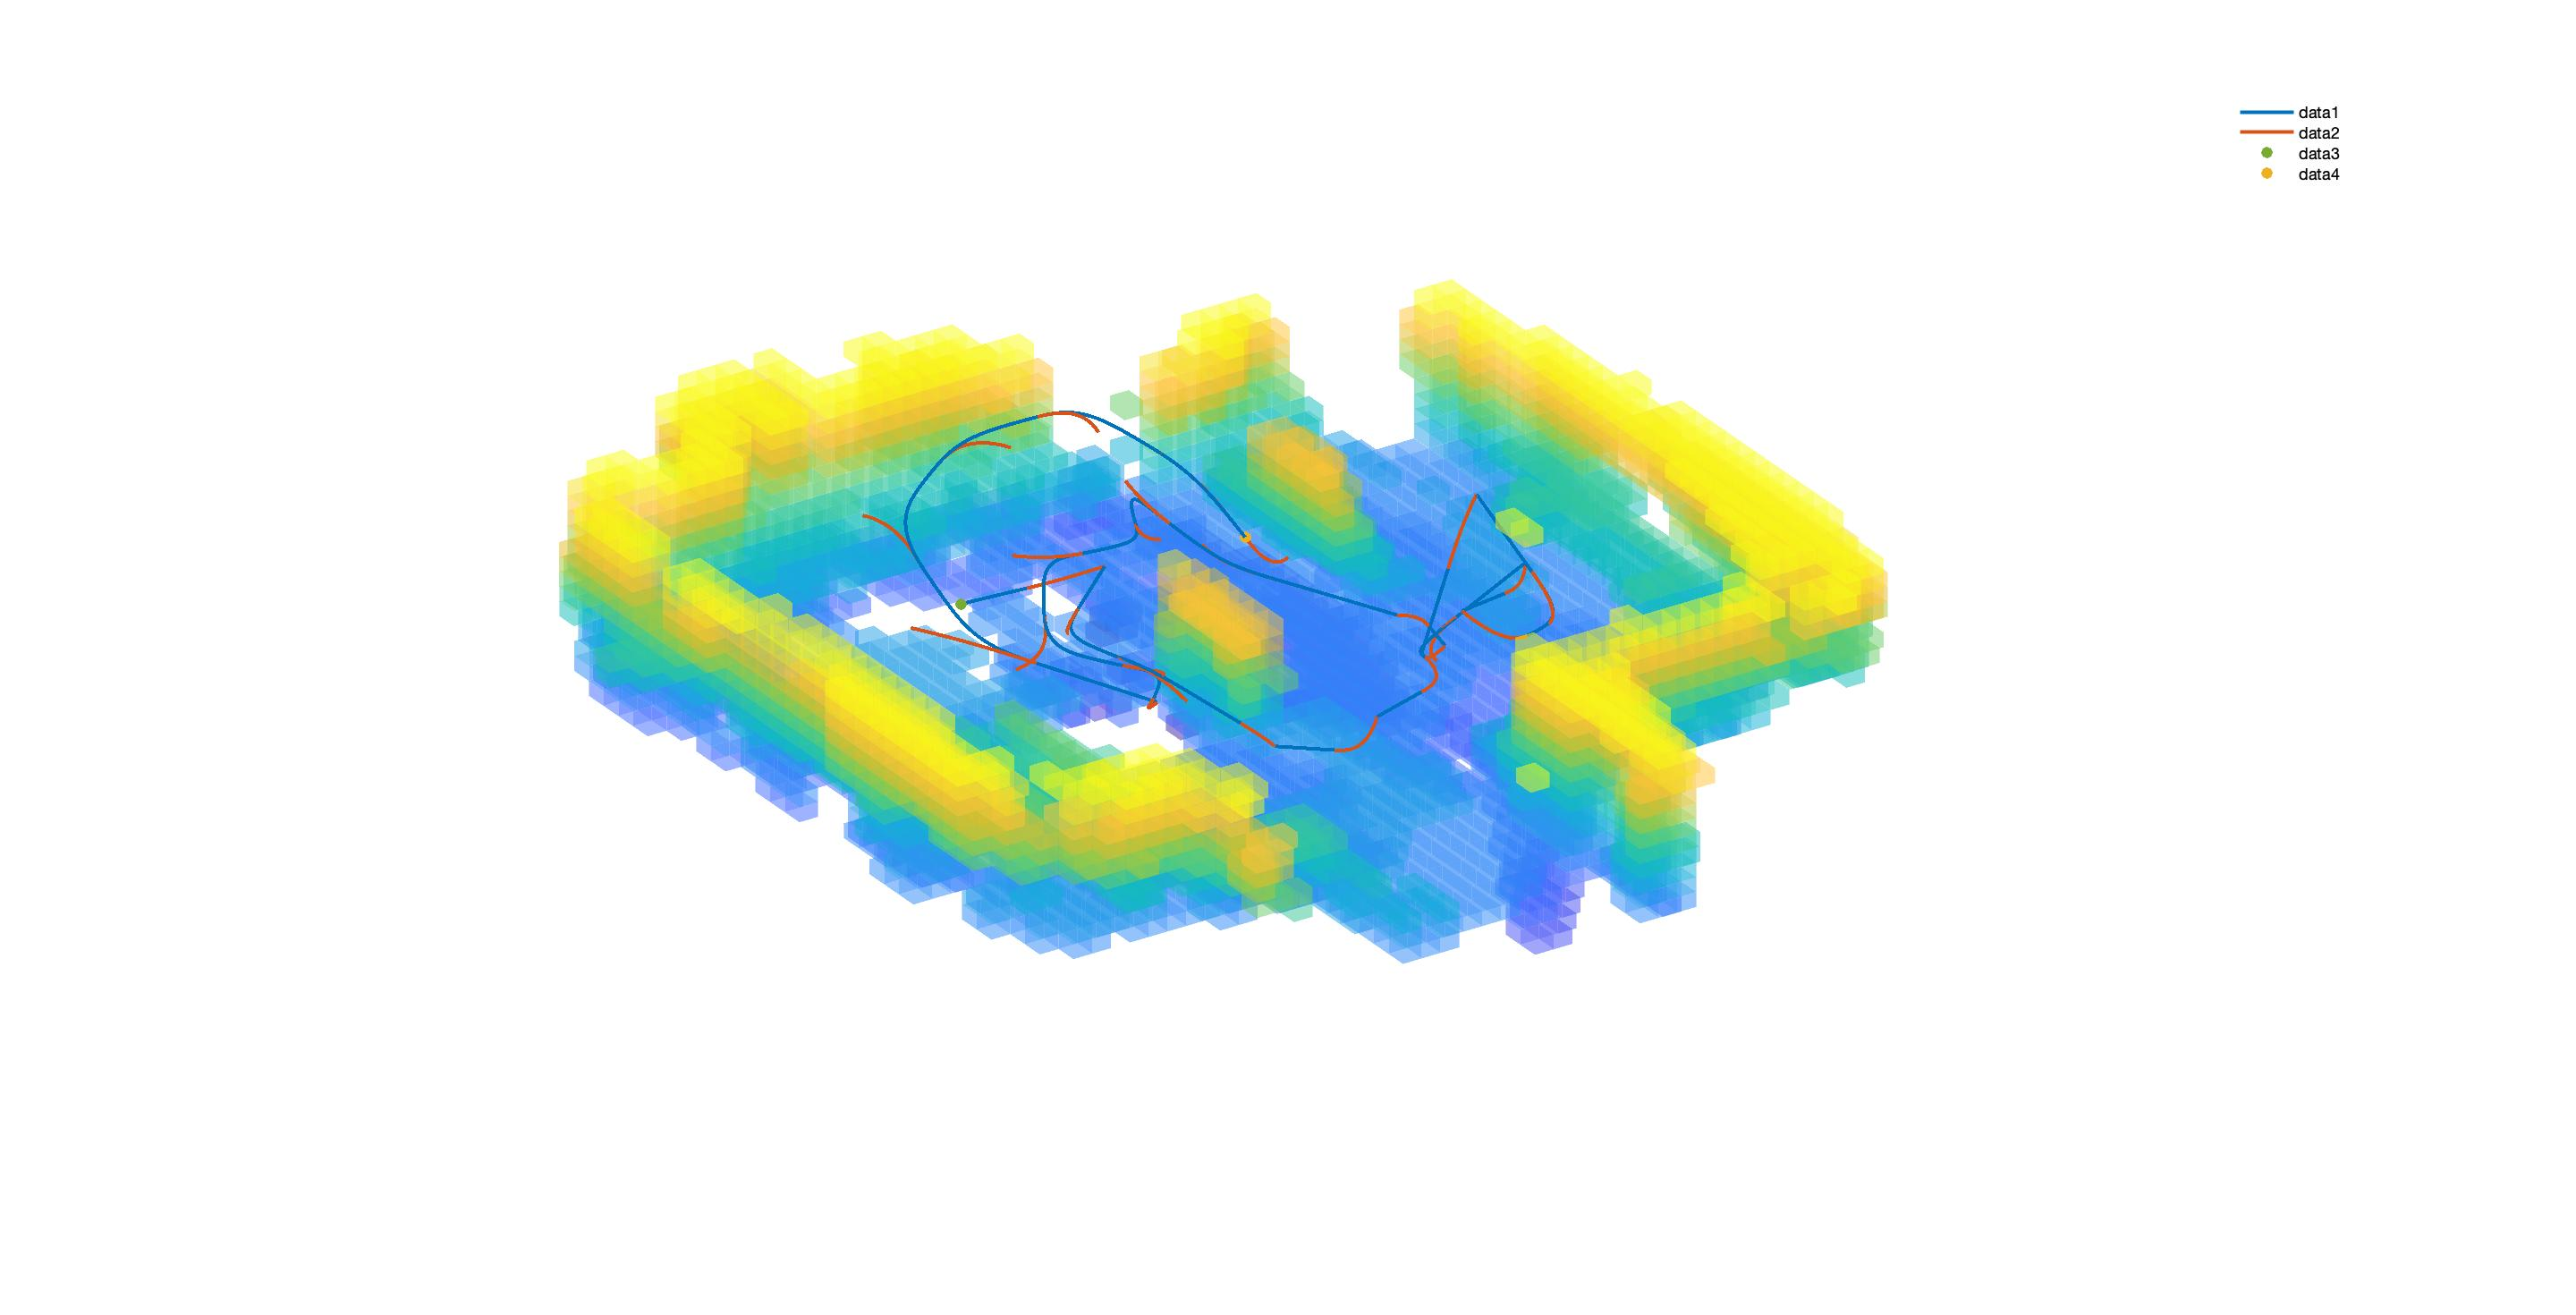
\includegraphics[trim={20cm 10cm 23cm 10cm}, clip = true, scale=.18]{Figs/Chapter4/full_exploration.jpg}
	\caption{Qualitative evaluation of the proposed method in a real-world experiment.
			The B\acuteacc ezier-based exploration succeeded in fast planning motion inside the unknown area
			without forcing zero end velocities and successfully avoiding the two obstacles
			placed at the center. In the figure, blue lines represent the reference trajectory, while in red
			are depicted the planned \emph{safe} maneuvers.}%
	\label{FIG:EXPLORATION-REAL-SCENARIO-RESULTS}
\end{figure}
\subsection{Reconstruction Gain, Trajectory Cost \& Total Utility}%
\label{SEC:EXPLORATION-COST-FUNCTIONS}
The algorithm presented in~\secref{SEC:EXPLORATION-TREE-UPDATE} is used to plan spatial trajectories by maximising
the total utility function $\loss(\cdot)$. As a consequence, since this function combines both node gain and cost,
the choice of functions $g(\cdot)$ and $c(\cdot)$, as well as $\loss(\cdot)$ itself, is crucial for the success of the exploration
procedure and of its performance. In this context, the reconstruction gain is defined as the amount of space that can be discovered
if the agent is located in the considered position ($\rr$) and oriented with a given heading angle ($\yaw$).
The function $g(\cdot)$ can be computed by casting rays outward from the sensor and summing up all the unmapped volume elements that
the ray crosses. Although there exist very efficient procedures useful to compute $g(\cdot)$, such as sparse
ray-casting~\cite{selin2019efficient}, its explicit evaluation is still the bottleneck for most of the exploration algorithms proposed
within the literature. The work~\cite{selin2019efficient}, motivated by the continuous nature of the reconstruction gain over its domain,
tries to overtake this problem by modelling it as a realisation of a Gaussian process~\cite{rasmussen2003gaussian}.
The idea is to infer, when possible, the gain value using previously sampled data, avoiding its explicit computation at each exploration
iteration. This approach has the limitation that when the process returns a \emph{poor} (in terms of resulting variance) estimation,
the gain must be explicitly re-computed, leading to a higher overhead due to the double computation. In this work we show that it is
possible to completely avoid the gain explicit computation in real-time, during the planning procedure, and it can be left as a background
thread. Unlike previous approaches, we propose to evaluate $g(\cdot)$ exclusively through Gaussian Process inference.
The motivating assumption is that in previously unexplored areas the reconstruction gain evaluates as the sensor FoV volume.
Therefore we impose a GP prior $g(\rr) \sim \mathcal{GP}(V_{\text{fov}}, k(\rr, \rr', \tau))$ consisting of a constant mean function,
equivalent to the sensor FoV volume, and a \emph{squared-exponential} kernel
\begin{equation*}
	\kf(\rr, \rr', \tau) = \exp \lp - \frac{\norm{\rr - \rr'}^2_2 }{2\tau^2} \rp,
\end{equation*}
where $\tau$ is a hyper-parameter known as \emph{characteristic length-scale}, iteratively estimated by minimising the associated log-likelihood
function~\cite{rasmussen2003gaussian}. The proposed approach alternates between gain prediction, using the currently sampled data and
the current estimation of the hyper-parameter, and correction, where $\tau$ is estimated by minimising the log-likelihood over the data.

In autonomous exploration applications, where classical RRT algorithms are employed, the trajectory cost is usually associated with node
distance~\cite{selin2019efficient, bircher2016receding}, or execution time~\cite{schmid2020efficient}. The former penalises long trajectories,
while the latter pushes the agent near its dynamical limits in order to execute the task as fast as possible. Recent studies about frontier
exploration~\cite{cieslewski2017rapid} have shown great results in terms of execution time and traveled distance. In these works, viewpoints
are selected considering minimal variations in velocity. Encouraged by the success of these algorithms and keeping in mind the necessity
to end the exploration as fast as possible, we propose a trajectory cost that weight execution time and total control effort.
The overall trajectory cost is formalised as
\begin{equation*}
	c \lp \CP^{\rr}_{i}, \CP^{\yaw}_{i}, \delta_{i} \rp =
		\mu_1 \delta_i + \mu_2 c_{\rr} \lp \CP^{\rr}_{i}, \delta_{i} \rp + \mu_3 c_{\yaw} \lp \CP^{\yaw}_{i}, \delta_i \rp,
\end{equation*}
where $\mu_{1:3}$ are tuning parameters, while $c_{\rr} \lp \cdot \rp$ and $c_{\yaw} \lp \cdot \rp$ take the following form
\begin{align}
	\label{EQ:EXPLORATION-TRAJ-COST-RR}
	c_{\rr} \lp \CP^{\rr}_i, \delta_i \rp & = \int_0^{\delta_i}  \norm{\frac{d^k \rr^i(\frac{\tau}{\delta_i})}{d\tau^k}}^2 d\tau, \\
	\label{EQ:EXPLORATION-TRAJ-COST-YAW}
	c_{\yaw} \lp \CP^{\yaw}_i, \delta_i \rp & = \int_0^{\delta_i}  \norm{\frac{d^p \yaw^i(\frac{\tau}{\delta_i})}{d\tau^p}}^2 d\tau.
\end{align}
In this particular case we selected $k = 2$ and $p = 1$, leading to trajectories with minimal accelerations and angular velocities.
Minimising the angular velocity has several benefits in terms of mapping reconstruction accuracy, due to the fact that
the captured data present low blur effect, especially when working with RGBD cameras. Note that the three components of
$\rr(\cdot) = [\ri_x(\cdot), \ri_y(\cdot), \ri_z(\cdot)]$ are decoupled inside the cost function, thus~\eqqref{EQ:EXPLORATION-TRAJ-COST-RR}
can be rewritten as
\begin{equation}%
	\label{EQ:EXPLORATION-COST-RR-DECOUPLED}
	c_{\rr} \lp \CP^{\rr}_i, \delta_i \rp = \sum_{j}^{x,y,z} \int_0^{\delta_i} \frac{d^k \ri^i_{j}(\frac{\tau}{\delta_i})}{d\tau^k}^2 d\tau.
\end{equation}
The Bernstein basis parameterisation is closed with respect to operations of derivative, power elevation and integral~\cite{farouki2012bernstein},
thus~\eqqref{EQ:EXPLORATION-TRAJ-COST-YAW} and~\eqqref{EQ:EXPLORATION-COST-RR-DECOUPLED} can be evaluated in closed form just acting on
the trajectory control points in the following way
\begin{align*}
    c_{\rr} \lp \CP^{\rr}_i, \delta_i \rp & =
	\begin{bmatrix}
		\rr^i_0 & \cdots & \rr^i_{n_{\rr}}
	\end{bmatrix}
	\basis_{\rr} \lp \delta_{i} \rp
	\begin{bmatrix}
		\rr^i_0 & \cdots & \rr^i_{n_{\rr}}
	\end{bmatrix}\T, \\
	c_{\yaw} \lp \CP^{\yaw}_i, \delta_i \rp & =
	\begin{bmatrix}
		\yaw^i_0 & \cdots & \yaw^i_{n_{\yaw}}
	\end{bmatrix}
	\basis_{\yaw} \lp\delta_i \rp
	\begin{bmatrix}
		\yaw^i_0 & \cdots & \yaw^i_{n_{\yaw}}
	\end{bmatrix}\T,
\end{align*}
where $\basis_{\rr}(\delta_{i})$ and $\basis_{\yaw}(\delta_{i})$ are the matrix form of the B\acuteacc ezier curves
$c_{\rr}(\cdot)$ and $c_{\yaw}(\cdot)$~\cite{qin2000general}. We take advantage of this property during the planning stage,
when selecting the remaining free points $\rr_3^i$, $\rr_4^i$ and $\yaw_2^i$. These are computed solving the following optimisation problem
\begin{equation*}
	\min_{\rr^i_3, \rr^i_4, \yaw^i_2} 
	\begin{bmatrix}
		\rr^i_0 \\ \vdots \\ \rr^i_{n_{\rr}} \\ \yaw^i_0 \\ \vdots \\ \yaw^i_{n_{\yaw}}
	\end{bmatrix}\T
	\begin{bmatrix}
		\mu_2 \basis_{\rr}(\delta_{i}) \\
		\mu_3 \basis_{\yaw}(\delta_i)
	\end{bmatrix}
	\begin{bmatrix}
		\rr^i_0 \\ \vdots \\ \rr^i_{n_{\rr}} \\ \yaw^i_0 \\ \vdots \\ \yaw^i_{n_{\yaw}}
	\end{bmatrix},
\end{equation*}
which results in an unconstrained QP problem, solvable by equalising the gradient to zero in a similar way as done in~\cite{richter2016polynomial}.
Finally, the total utility function, responsible to merge gains and costs of the tree nodes in only one utility value, has been chosen 
borrowing the idea of~\cite{schmid2020efficient} that proposes a total utility function based on the notion of efficiency
\begin{equation*}
	\loss \lp \RR(\node_i) \rp = \frac{\sum_{\node_l \in \RR \lp \node_i \rp} g_l}{\sum_{\node_l \in \RR \lp \node_i \rp} c_l}.
\end{equation*}

\subsection{Implementation Details}%
\label{SEC:EXPLORATION-IMPLEMENTATION-DETAILS}
%%%%%%
\begin{figure}[!t]
	\centering
	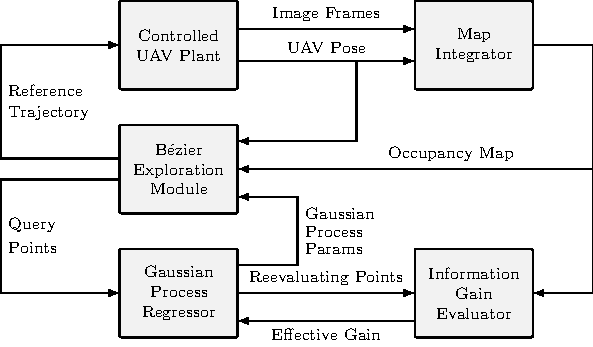
\includegraphics[scale=.9]{Figs/Chapter4/alg_scheme.pdf}
	\caption{The overall scheme of the proposed exploration system.}%
	\label{FIG:EXPLORATION-ALG-SCHEME}
\end{figure}
%%%%%%
The overall structure of the proposed framework is shown in \figref{FIG:EXPLORATION-ALG-SCHEME}. The planning framework is built on top
of a reliable UAV control scheme and an occupancy map integrator whose construction is out of the scope of this chapter.
The solution relies on three different threads running in parallel.
\begin{enumerate}
	\item \emph{Exploration Module}.\\
	This thread acts as the exploration supervisor and is in charge of computing the reference trajectories to be executed from
	the UAV platform. The exploration module continuously grows and maintains the trajectories tree via random sampling and by
	reevaluating each sampled non-executed node at each new iteration. Since the tree is executed in a receding-horizon fashion,
	every time a new trajectory is commissioned, a bunch of previously planned trajectories may become infeasible due to continuity
	issues. To handle this problem an activation flag is added as a node property. Note that at each sampling, only the active branches
	are taken into consideration. Furthermore, the explorer node also keeps care about possible \emph{deadline violations}.
	In these cases the executed safe trajectory is added to the tree and rewired to all nearby active nodes.
	This prevent us to lose previous sampled possible promising trajectories.
	\item \emph{Gaussian Regressor}.\\
	This thread receives all sampled points from the exploration module and implements a policy to allow the cache of only the most
	informative ones. In particular, a new point is retained only if it belongs to a new and not explored area. The implementation of a
	R-tree structure allows for fast point insertion and retrieval, moreover it eases the insertion condition check. In order to be
	consistent with the exploration task, and the evolution of the known map, all cached points are reevaluated periodically via
	explicit gain computation. Such a module is in charge to train the Gaussian process parameters used by the explorer.
	\item \emph{Information Gain Evaluator}.\\
	This thread receives the evaluating point and computes explicitly the information gain via sparse ray-casting as in~\cite{selin2019efficient}.
\end{enumerate}
The architectural subdivision of the implemented algorithm in three different threads allows fast computing high informative trajectories
\graffito{The implemted code is open-source and completely available at the GitHub repository github.com/casy-lab/BezierFastExploration.}
without the explicit gain computation bottleneck. The whole algorithm has been implemented as a ROS network and paired with the PX4
autopilot both for the software-in-the-loop simulations and the real-world tests. As a map representation we use OctoMap~\cite{hornung2013octomap}.
%%%%%%%%%
{
\renewcommand{\arraystretch}{1.35}
\begin{table}[b!]
    \centering
    \begin{tabular}{||c|c||c|c||}
        \hline
        \hline
        Max Vel. & $1.5 m/s$ & Max Acc. & $1.5 m/s^2$ \\
        \hline
        Sampled Nodes & $40$ & Max Length & $3 m$ \\
        \hline
        Min Range & $0.3 m$ & Max Range & $5.0 m$ \\
        \hline
        Camera FoV & $115\times60$ deg & Map Res. & $0.2 m$ \\
        \hline
        $\mu_1$ $\mu_2$ $\mu_3$ & $0.5$ $0.1$ $0.1$ & Time Res. & $0.5 s$ \\
        \hline
        Min Time & $1s$ & Max Time & $5s$ \\
        \hline
        \hline
    \end{tabular}
    \caption{Parameters used in simulations.}%
	\label{TAB:EXPLORATION-SIMULATION-PARAMETERS}
\end{table}
%%%%%%%%%
%%%%%%%%%
\begin{table}[b!]
    \centering
    \begin{tabular}{||c|c||c|c||}
        \hline
        \hline
        Max Vel. & $0.5 m/s$ & Max Acc. & $0.5 m/s^2$ \\
        \hline
        Sampled Nodes & $20$ & Max Length & $3 m$\\
        \hline
        Min Range & $0.3 m$ & Max Range & $3.0 m$ \\
        \hline
        Camera FoV & $87\times58$ deg & Map Res. & $0.2 m$ \\
        \hline
        $\mu_1$ $\mu_2$ $\mu_3$ & $0.5$ $0.1$ $0.1$ & Time Res. & $0.5 s$ \\
        \hline
        Min Time & $1s$ & Max Time & $5s$ \\
        \hline
        \hline
    \end{tabular}
    \caption{Parameters used in the real-world experiments.}%
	\label{TAB:EXPLORATION-REAL-PARAMETERS}
\end{table}
}
%%%%%%%%%%%
\subsection{Experimental Evaluation}%
\label{SEC:EXPLORATION-EXPERIMENTAL-EVALUATION}
The proposed approach has been evaluated via Gazebo-based simulations, exploiting the environment RotorS~\cite{furrer2016rotors} along with
the provided 3DR Iris quadrotor model, endowed of a depth sensor. The algorithm performance have been also qualitatively evaluated in
real-world scenario tests. In all tests the agent starts in the origin with zero yaw angle. The agent performs an initial rotation
of $360$ degrees around the initial hovering point in order to be sure to start the exploration with some initial information at hand.
%%%%%%%%%%
\begin{figure}[!t]
	\begin{center}
		\begin{minipage}{.4\linewidth}
			\centering
			\subfloat[]{%
				\label{FIG:EXPLORATION-SIM-TEST-A}%
				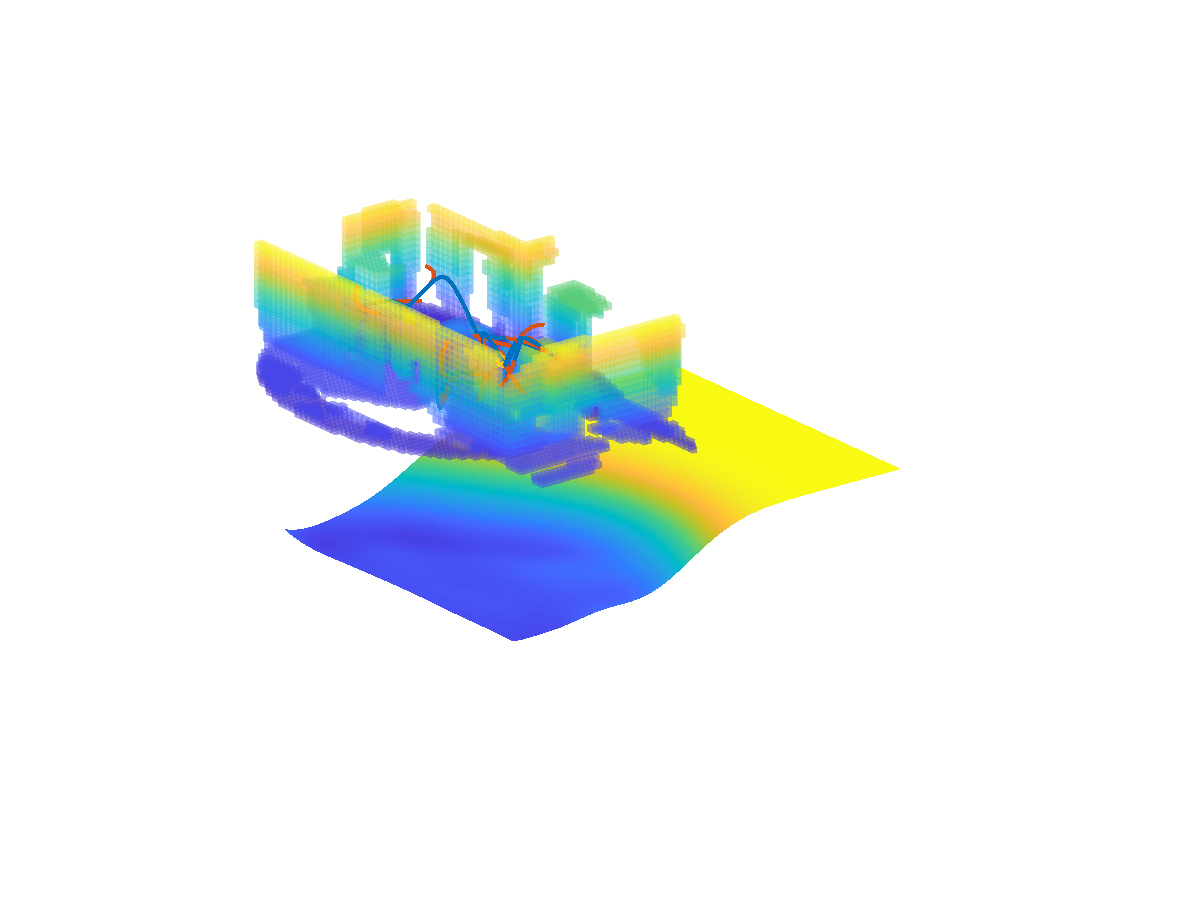
\includegraphics[trim={3cm 1.5cm 3cm 1cm}, clip = true, width = 1.2\textwidth]{Figs/Chapter4/exploration_100s.eps}}
		\end{minipage}
		\begin{minipage}{.4\linewidth}
			\centering
			\subfloat[]{%
				\label{FIG:EXPLORATION-SIM-TEST-B}%
				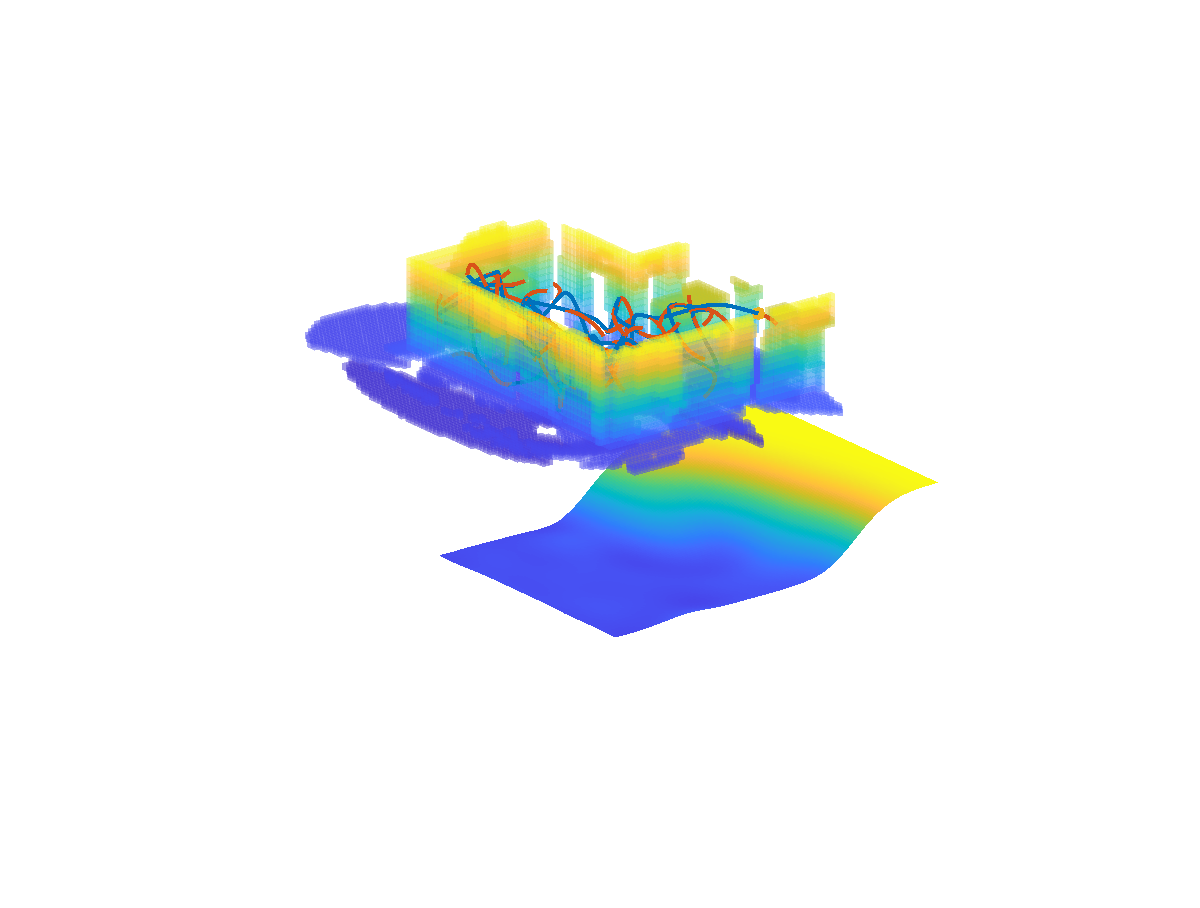
\includegraphics[trim={5cm 1.5cm 3cm 1cm}, clip = true, width = 1.2\textwidth]{Figs/Chapter4/exploration_200s.eps}}
		\end{minipage}
		\begin{minipage}{.4\linewidth}
			\centering
			\subfloat[]{%
				\label{FIG:EXPLORATION-SIM-TEST-C}%
				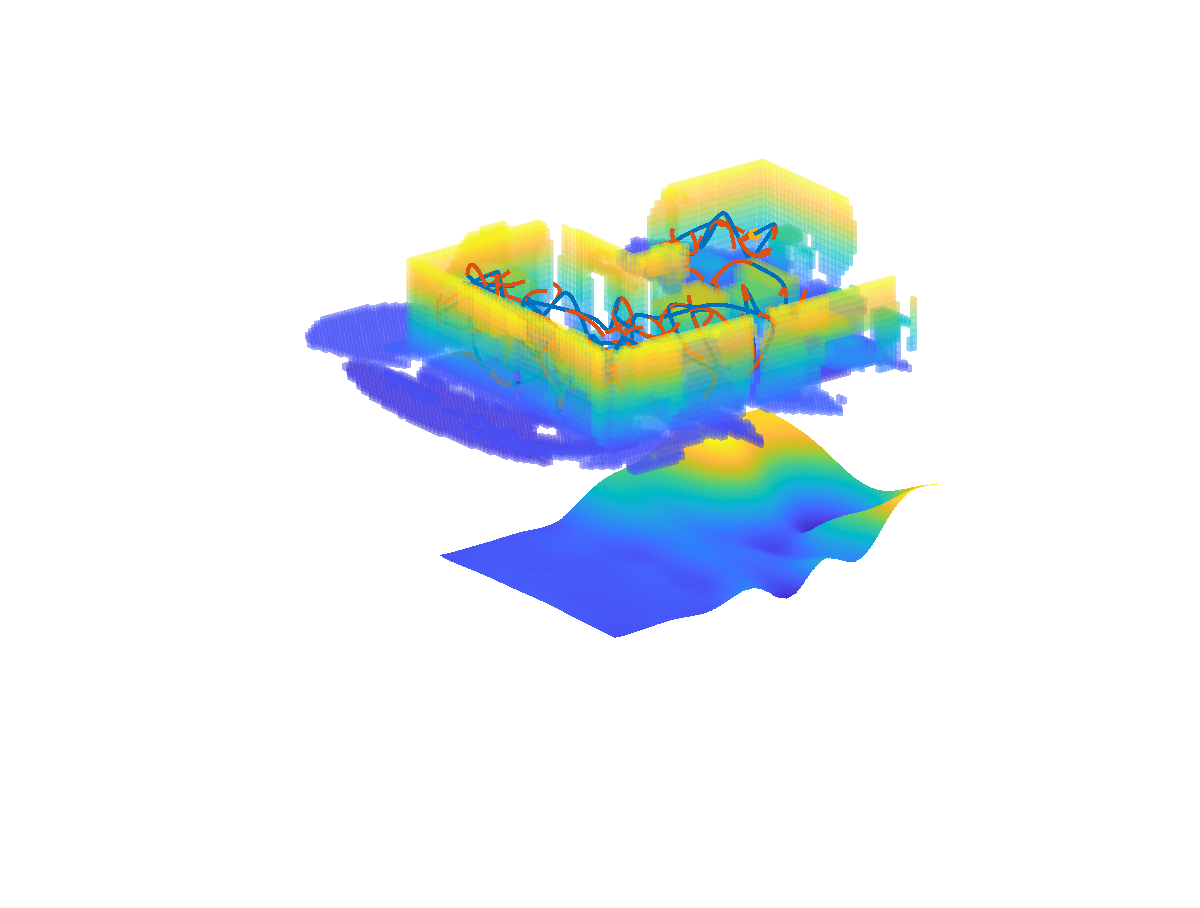
\includegraphics[trim={5cm 1.5cm 3cm 1cm}, clip = true, width = 1.2\textwidth]{Figs/Chapter4/exploration_300s.eps}}
		\end{minipage}
	\end{center}
	\caption{Results of the simulation tests. The exploration algorithm runs over a map of $20\times10\times3$
	meters and was able to complete the exploration after only $400$ seconds. In the image, in order,
	(a) exploration state at $100$ seconds, (b) exploration state at $200$ seconds, and (c) exploration state at $300$ seconds.
	At the bottom of each time snapshot, a visual representation of the Gaussian inferred information gain is reported.
	}\label{FIG:EXPLORATION-SIM-TEST}
\end{figure}
%%%%%%%%%%
%%%%%%%%%%
\begin{figure}[!t]
	\begin{center}
		\begin{minipage}{.4\linewidth}
			\centering
			\subfloat[]{%
				\label{FIG:EXPLORATION-REAL-TEST-A}%
				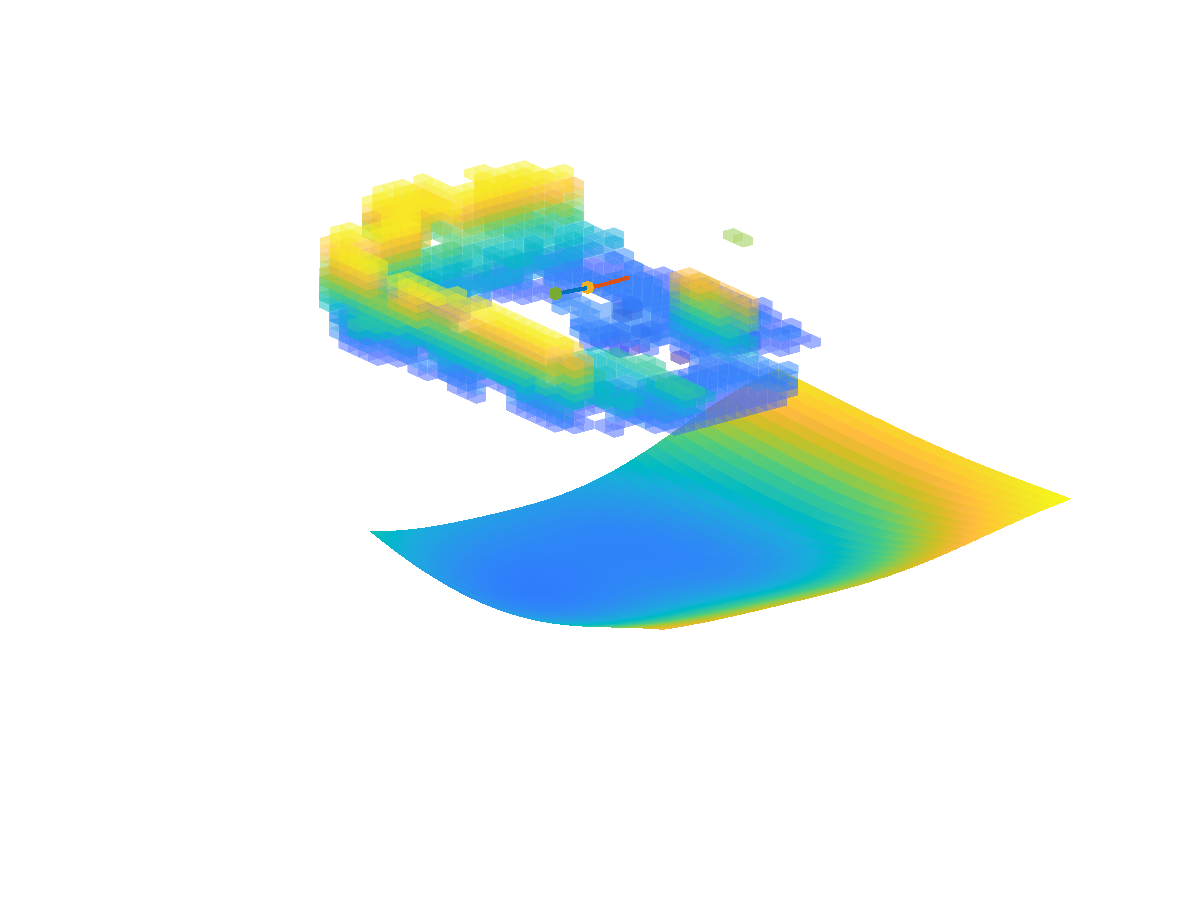
\includegraphics[trim={5cm 1.5cm 2cm 2.2cm}, clip = true, width = 1\textwidth]{Figs/Chapter4/20s.eps}}
		\end{minipage}
		\begin{minipage}{.4\linewidth}
			\centering
			\subfloat[]{%
				\label{FIG:EXPLORATION-REAL-TEST-B}%
				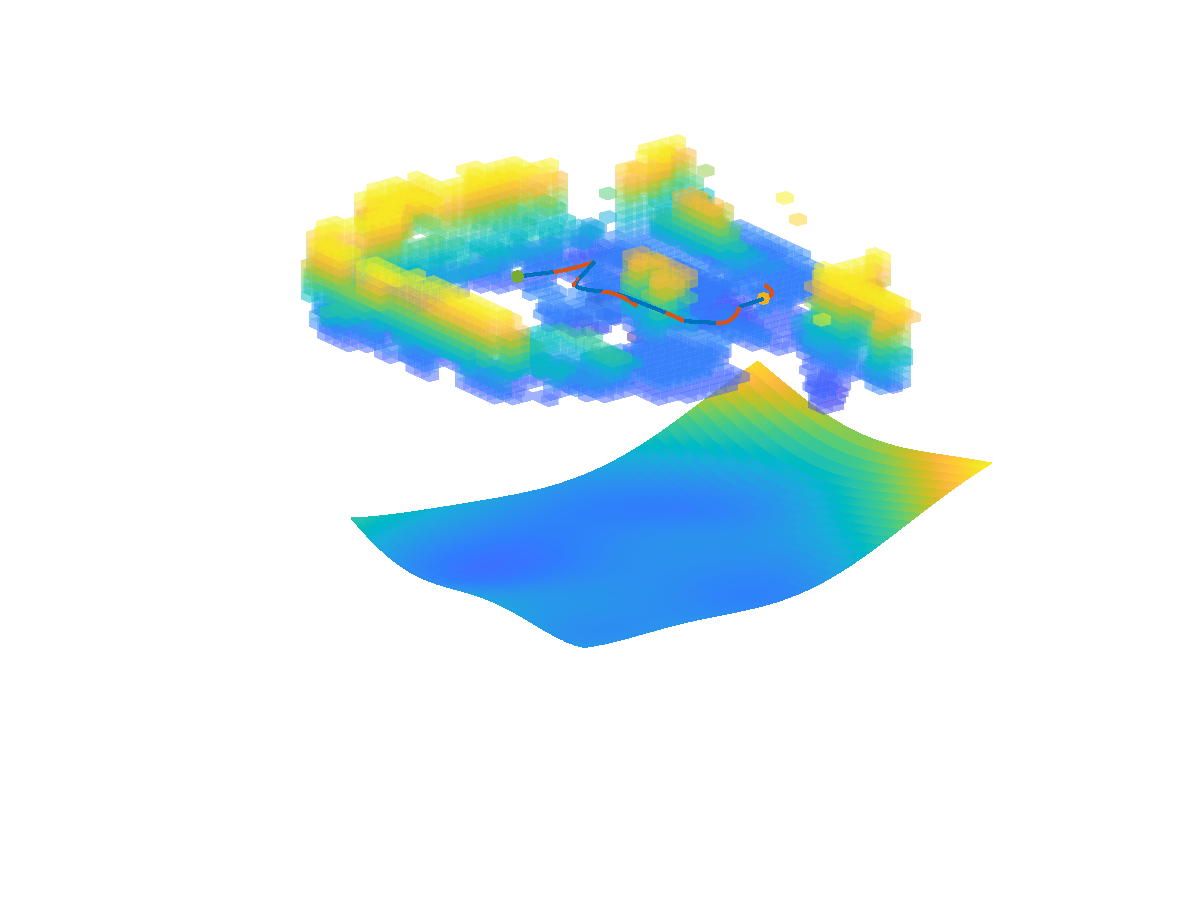
\includegraphics[trim={5cm 1.5cm 3cm 2.2cm}, clip = true, width = 1\textwidth]{Figs/Chapter4/57s.eps}}
		\end{minipage}
		\begin{minipage}{.4\linewidth}
			\centering
			\subfloat[]{%
				\label{FIG:EXPLORATION-REAL-TEST-C}%
				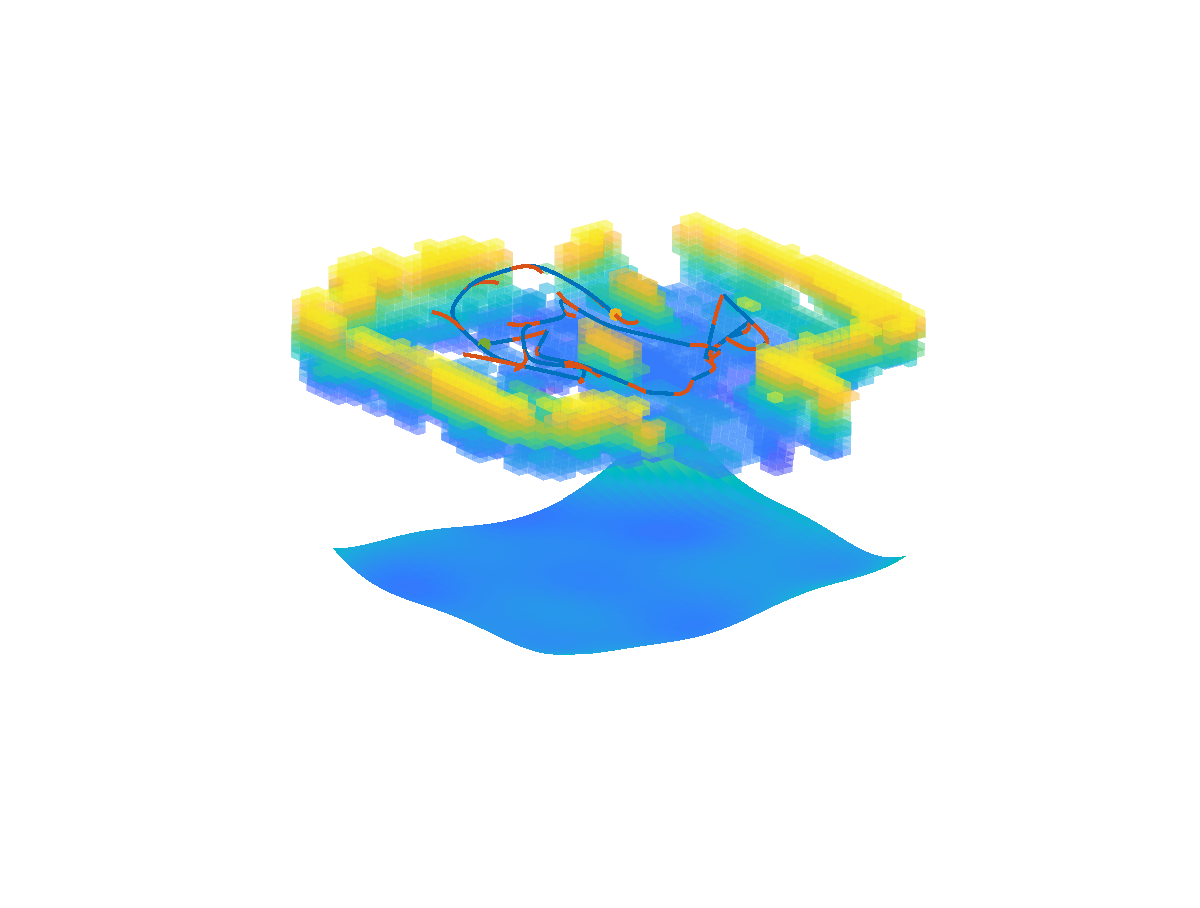
\includegraphics[trim={5cm 1.5cm 3cm 2.2cm}, clip = true, width = 1\textwidth]{Figs/Chapter4/167s.eps}}
		\end{minipage}
	\end{center}
	\caption{Results of the real-world exploration test. The exploration algorithm was run using only integrated onboard
	sensors and computational capabilities. In the image, in order, (a) exploration state at $20$ seconds,
	(b) exploration state at $57$ seconds, and (c) exploration state at $167$ seconds.
	At the bottom of each time snapshot, a visual representation of the Gaussian inferred information gain is reported.
	}\label{FIG:EXPLORATION-REAL-TEST}
\end{figure}
%%%%%%%%%%
The parameters used during the simulation tests are reported in~\tabref{TAB:EXPLORATION-SIMULATION-PARAMETERS}.~\figref{FIG:EXPLORATION-SIM-TEST}
shows the obtained simulation results when agent is required to map an $20\times10\times3$
urban canyon. In particular, in~\figref{FIG:EXPLORATION-SIM-TEST}, the blue lines represent the reference trajectory, the red
ones are the planned safe motions (both executed and non-executed), while the bottom surface represents the current Gaussian
process state. It can be noticed that, the Gaussian process is constantly kept updated with the current map information and it
results to be consistent, at each time instant, with the exploration task. In order to evaluate the performances against the
state-of-the-art solutions, the proposed algorithm has been compared with the \emph{Autonomous Exploration Planner} (AEP)
described in~\cite{selin2019efficient}.~\figref{FIG:EXPLORATION-COMPARED-ALGOROTHMS} compares the amount of explored volume
over time by both the approaches. The blue line represents the average of explored area obtained deploying our approach over $10$
experiments, with the associated standard deviation represented in shaded blue. Conversely, the line and shade red reports the
results obtained via AEP, with the global exploration module disabled, on the same number of experiments. It can be noticed that
both algorithms achieve comparable results at the beginning of the exploration, where most of the volume needs to be explored,
then our solution tends to get higher exploration rate, thanks to the ability to fast plan the next trajectory. Moreover, it is
worth noting that our solution provides more consistency between different tests, as the variance is narrower with respect to the AEP,
thus guaranteeing better repeatability of the experiment and a mitigation of the worst case scenarios.
\figref{FIG:EXPLORATION-TRAVELLED-DISTANCE} depicts the overall travelled distance on same experiments. Since our solution plans
trajectories by never stopping the UAV motion, this leads to an overall travelled distance $2$ times higher than the AEP solution.
%%%%%%%%%%%
\begin{figure}[!t]
	\centering
	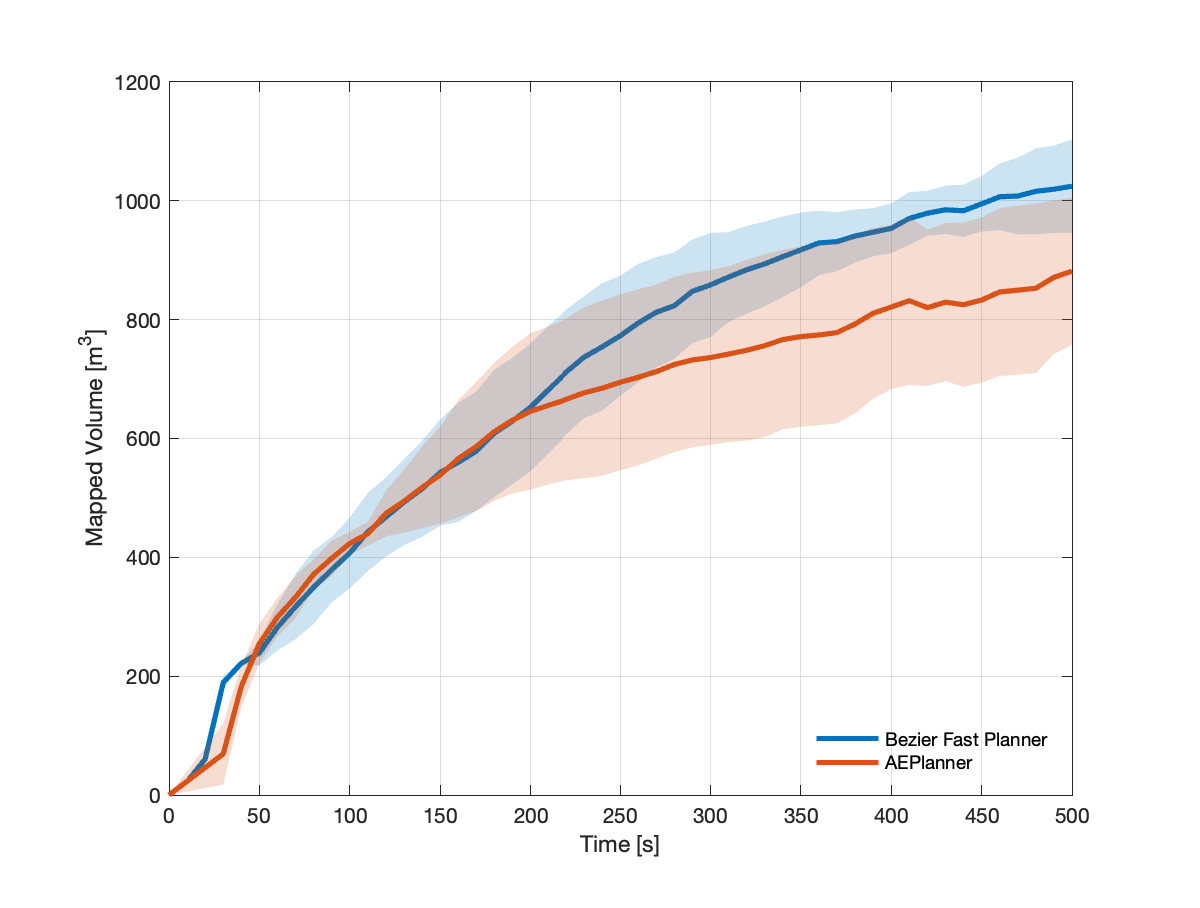
\includegraphics[trim={0cm 0cm 0cm 1cm}, clip = true, scale=.4]{Figs/Chapter4/mapped_volume.eps}
	\caption{Exploration progress for the urban $20 \times 10 \times 3$ canyon. Mean and standard deviation over $10$
	experiments are shown. Notice that due to the employing of pierced nets as maps borders makes the overall explored
	volume higher than the real volume.}%
	\label{FIG:EXPLORATION-COMPARED-ALGOROTHMS}
\end{figure}
\begin{figure}[!t]
	\centering
	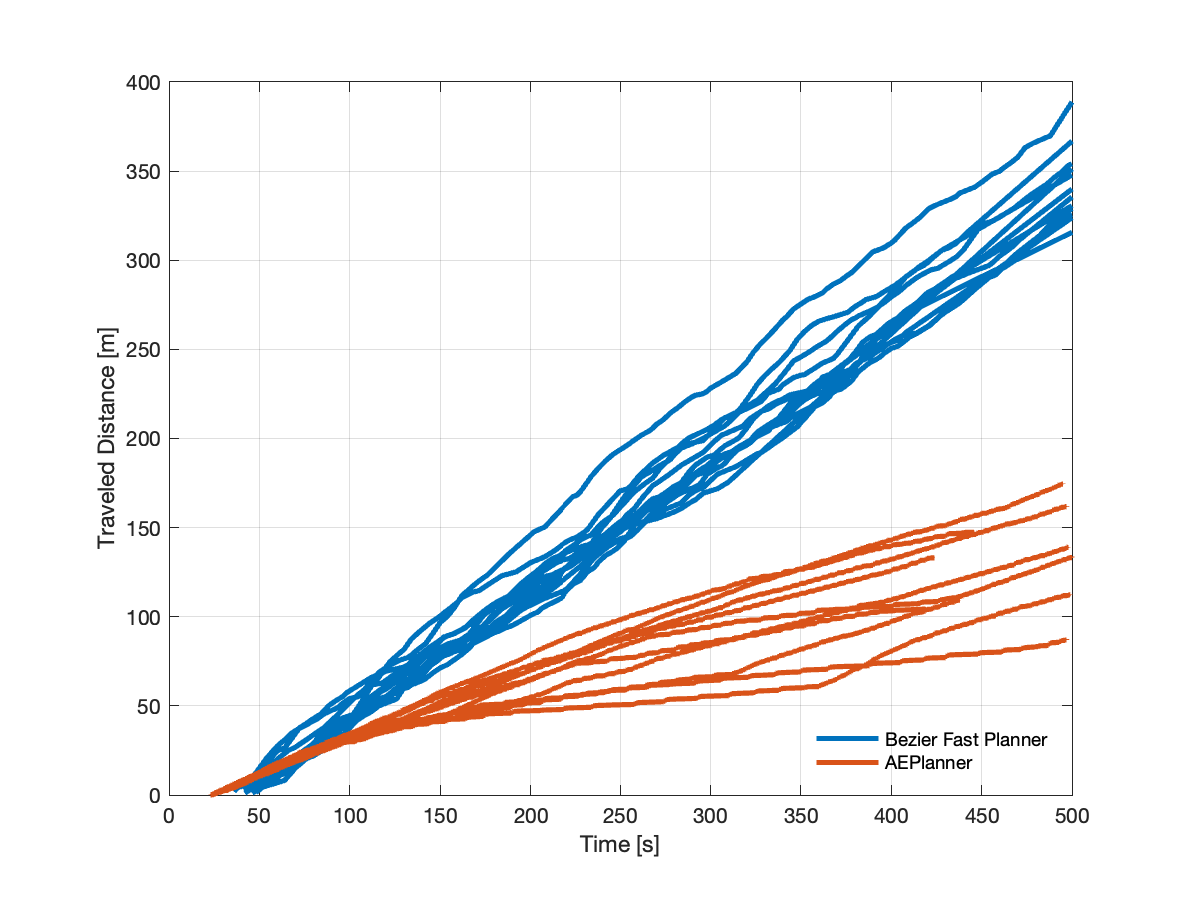
\includegraphics[scale=.4]{Figs/Chapter4/traveled_distance.eps}
	\caption{Overall traveled distance in the urban canyon. The traveled distances over $10$ experiments are shown.}%
	\label{FIG:EXPLORATION-TRAVELLED-DISTANCE}
\end{figure}
%%%%%%%%%%%
The solution has been tested using a real UAV inside an indoor scenario using our office spaces.
The obtained results are depicted in~\figref{FIG:EXPLORATION-REAL-TEST}. The used parameters are reported
in~\tabref{TAB:EXPLORATION-REAL-PARAMETERS}. The available area was $9\times6\times2.5$ meters and it was successfully
mapped in $170$ seconds, the maximum camera range was saturated at $3$ meters in order to stress navigation trajectories around
obstacles. The used UAV was powered by the PX4 autopilot and endowed with a depth Intel RealSense D455 camera, mounted frontally.
Visual odometry, used to localize the UAV in the indoor scenario, was provided by an Intel Realsense T265 tracking camera. 

%----------------------------------------------------------------------------------------
\section{Patrolling: A Different Exploration Perspective}%
\label{SEC:SEARCH-PATROLLING-PERSPECTIVE}
In this section, we review a novel and different solution to the exploration problem stated in~\secref{SEC:EXPLORATION-PROBLEM-DEFINITION},
in the setting where the environment is completely known and the only goal is to find out interesting points, or objects,
inside the explored area. In this framework, the general exploration problem can be specialised by considering a third attribute, jointly
with \emph{free} and \emph{occupied}, namely \emph{interest}. A subset of the overall volume $\V \in \R^3$ will be categorised as
$\V_{\text{int}} = \{ \xx \in \V \mid \Gamma(\xx) = \text{int} \}$, thus the exploration task will be considered complete when
$\V_{\text{free}} \cup \V_{\text{occ}} \cup \V_{\text{int}} = \V \setminus \V_{\text{res}}$, with $\V_{\text{free}}$, $\V_{\text{occ}}$,
and $\V_{\text{res}}$ defined as in~\secref{SEC:EXPLORATION-PROBLEM-DEFINITION}.
Let us suppose to completely apriori known the set $\V_{\text{free}}$, then the exploration goal reduces to correctly classify
$\V \setminus \V_{\text{res}} \setminus \V_{\text{free}}$ between $\V_{\text{occ}}$ and $\V_{\text{int}}$.
The proposed approach is based on the idea that the employed software pipeline used to recognise the objects of interest may fail
in doing that, and the probability of failure is jointly linked with the capability of the endowed sensor. Moreover, the autonomous
platform may not be able to perform the commissioned motion due to environment modifications, or unexpected and unmapped obstacles.
The stochastic nature of the problem at hand, along with the stochasticity of the adopted pipeline, embraces a purely probabilistic
approach, so the locations of the objects are expressed in a likelihood form, that in the following takes the name of
\emph{probabilistic map}.

Similar to the algorithm described in~\secref{SEC:EXPLORATION-LARGE-SCALE}, the core of the proposed solution consists of an RRT of
possible and feasible motions. Unlike the previous approach, here we do not constrain the tree to directly represents pieces of
possible trajectories. In this case, the tree is built to describe possible collision-free paths inside the environment, while the
computation of the associated timing laws is left as next step, during the \emph{trajectory optimisation} stage. In this view,
the timing law is selected to ensure trajectory feasibility in terms of induced maximum velocity and acceleration.
The tree expansion is supplied with the aforementioned probabilistic map, which is copied and kept updated on each new sampled
node. The extension of the node attributes set with a copy of the current likelihood map allows for time consistency.
The map in each node is in fact constantly kept updated, allowing for cost increase or decrease if the exploration time grows, or 
if a particular node has been visited, respectively.
The remainder of this section unfolds as follows~\secref{SEC:SEARCH-MAP-STRATEGY} and~\secref{SEC:SEARCH-COMPLEXITY-REDUCTION}
deeply analyze the aforementioned mapping strategy, bridging the gap between discrete and continuous maps, and proposing a novel
mapping framework. In~\secref{SEC:SEARCH-TREE-STRUCTURE} the tree structure is briefly described, along with the adopted growth
policy,~\secref{SEC:SEARCH-TRAJECTORY-OPTIMISATION} introduces the used time allocation procedure and how the final trajectory is iteratively
refined before its commissioning. Finally,~\secref{SEC:SEARCH-EXPERIMENTAL-RESULTS} reports the obtained results when the proposed
approach is exploited to perform target search in a completely known environment.

\subsection{Mapping Strategy}%
\label{SEC:SEARCH-MAP-STRATEGY}
%%%%%%%%%%%
\begin{figure}[!t]
	\centering
	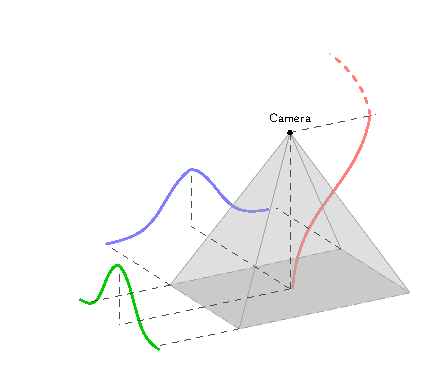
\includegraphics[width=0.8\textwidth]{Figs/Chapter4/camera_fov.pdf}
	\caption{Probabilistic adopted camera model.}
	\label{FIG:SEARCH-CAMERA-MODEL}
\end{figure}
%%%%%%%%%%%
In this solution we employ a discrete occupancy-based mapping approach~\cite{hornung2013octomap} to store information about occupied
and free spaces, while interesting environment features, or objects, are stored by following a continuous probability mapping paradigm.
In particular, Gaussian processes are used to infer the belief of features existence. This approach allows to increase the map
reliability by introducing spatial correlations between data while maintaining the memory consumption low, and to formulate an information
gain that trades-off between target re-observation and exploration for new ones.
In a probabilistic framework, the target positions are usually represented through a set of discrete random variables defined over a
discretization of the search space ($\E \subset \R^3$). This approach leads to a discrete occupancy map ($\M$) where each grid cell is associated with
an independent Bernoulli random variable ($\bernoulli_i$) whose Probability Mass Function (PMF) represents the probability of target
occupancy~\cite{popovic2020informative}
\begin{equation*}
	\Prob \lp \bernoulli_i = k \rp =
	\begin{cases}
		\prob_i &\text{if } k=1, \\
		1 - \prob_i &\text{if } k=0.
	\end{cases}
\end{equation*}
The value of $\prob_i$ for each $\bernoulli_i \in \M$ inside the sensor FoV is updated, at each new sensor measurement,
via the Bayes formula
\begin{equation*}
	\Prob \lp \bernoulli_i \mid z^{1:t}, s^{1:t} \rp = \frac{\Prob \lp z^{t} \mid \bernoulli_i, s^t \rp
													   \Prob \lp \bernoulli_i \mid z^{1:t-1}, s^{1:t-1} \rp}{\Prob \lp z^t \rp},
\end{equation*}
where $z^t$ is the current observation at sensor position $s^t$. The aforementioned relation is usually rewritten in
log-likelihood notation, where products are replaced by additions, allowing for faster updates~\cite{hornung2013octomap}
\begin{equation}
	\label{EQ:SEARCH-LOG-LIKELIHOOD}
	\like \lp \bernoulli_i \mid z^{1:t}, s^{1:t} \rp = \like \lp \bernoulli_i \mid z^{1:t-1}, s^{1:t-1} \rp +
													   \like \lp z^t \mid \bernoulli_i, s^t \rp,
\end{equation}
with
\begin{equation*}
	\like \lp \bernoulli_i \rp = \log \lp \frac{\Prob \lp \bernoulli_i = 1 \rp}{1-\Prob \lp \bernoulli_i = 1 \rp} \rp.
\end{equation*}
In~\eqqref{EQ:SEARCH-LOG-LIKELIHOOD} the quantities $\like \lp \bernoulli_i \mid z^{1:t-1}\rp$ and
$\like \lp \bernoulli_i \mid z^{1:t}\rp$ represent the prior and posterior probability, respectively.
While, $\like \lp z^t \mid \bernoulli_i \rp$ is the observation likelihood that strongly depends on the adopted probabilistic
sensor model. In our specific case, we employ a downward-facing monocular camera to detect targets on the ground,~\figref{FIG:SEARCH-CAMERA-MODEL}
shows the probabilistic model for such type of sensor. The probability to retrieve correct measures decreases approaching the FoV boundaries,
as well as the maximum distance allowed. This kind of behavior is well described by a modified logistic function of the kind
\begin{equation*}
	\Prob \lp z^t = 1 \mid \bernoulli_i, s^t \rp = 0.5 + \frac{\prob_{\text{max}}}{1 + \exp \lp \norm{x_i - s^t}_{W} - c \rp},
\end{equation*} 
where $x_i \in \M$ represents the grid cell associated with $\bernoulli_i$, while $s^t \in \R^3$ is the current sensor position.
The weight matrix $W \in \R^{3 \times 3}$, and the parameters $\prob_{\text{max}}$ and $c$ are responsible to shape the function
over the camera field of view.

Despite the power of discrete maps, in our solution we choose to adopt a continuous mapping strategy.
Continuous maps allow to incorporate spatial correlations of input data and, potentially, require lower memory to maintain the overall map.
These advantages are not for free since continuous maps present a higher computational complexity. Gaussian processes are well suited for
this purpose since can encode spatial correlations in a probabilistic way and, with a careful choice of training points, take low
computational and storage memory. With this idea in mind, the log-likelihood of occupancy is treated, in this case, as a continuous
function over the search space $\like:\E \subset \R^3 \mapsto \R$. The key idea is to model such function as a realization of a Gaussian
process. A GP model is completely defined by a mean function $\prior \lp \xx \rp: \E \mapsto \R$ and a covariance function
$\kf \lp \xx, \xx' \rp: \E \times \E \mapsto \R$
\begin{align*}
	\like \lp \xx \rp \sim \GP \lp \prior \lp \xx \rp, \kf \lp \xx,\xx' \rp \rp.
\end{align*}
Although there are many possible choices for mean and covariance functions, usually the structure of $\prior$ and $\kf$ are assumed to be
known up to certain hyper-parameters ($\prior \lp \cdot, \param_{\prior} \rp$, $\kf \lp \cdot, \param_{\kf} \rp$).
In the particular case of target search, the mean function should be chosen on the basis of some a prior notions about the target existence,
thus it is a priori fixed and does not depend on any hyper-parameter. In those cases in which no prior information is available,
the mean function is simply $\prior \lp \xx \rp = 0$  $\forall \xx \in \E$, that corresponds to an occupancy probability of $0.5$.
The covariance function, aka \textit{kernel}, influences the GP behavior when fed with training data points.
The results presented afterward are obtained using a \textit{Matérn $3/2$ kernel}, that takes the form
\begin{equation*}
	\kf  \lp \xx, \xx', \param \rp = \lp 1 + \frac{\sqrt{3} d}{\param} \rp \exp \lp - \frac{\sqrt{3} d }{\param} \rp, 
\end{equation*}
where $d = \norm{\xx - \xx'}^2_2$, while $\param$ is a hyper-parameter known as \textit{characteristic length-scale}~\cite{rasmussen2003gaussian}.
The Matérn $3/2$ kernel is very common in geostatistical analysis, due to its capability to capture discrete targets~\cite{meera2019obstacle},
thus it results very suitable also for this particular application. Given $\nsample$ noisy observations $\yy^{1:\nsample} \in \R^{\nsample}$
and the respective sampling locations $\xx^{1:\nsample} \in \R^{\nsample \times 3}$, the posterior distribution of $\like$ is a Gaussian distribution,
whose mean and variance can be evaluated as
\begin{align}%
	\label{EQ:SEARCH-POST-MEAN}
	\pmu \lp \xx \rp & = \prior \lp \xx \rp + \kv \lp \xx \rp\T \lps \km + \nn I \rps^{-1}
						 \lp \yy^{1:\nsample} - \prior \lp \xx^{1:\nsample} \rp \rp, \\
	\label{EQ:SEARCH-POST-VARIANCE}
	\pvar \lp \xx \rp & = \kf \lp \xx,\xx \rp - \kv \lp \xx \rp\T \lps \km + \nn I \rps^{-1} \kv \lp \xx \rp.
\end{align}
To deal with the unknown hyper-parameter, we follow an empirical Bayes approach~\cite{benevento2020multi}, where the prediction steps are
alternated with parameters estimation steps via maximum likelihood
\begin{equation*}
	\param = \arg\max_{\param}  \prob \lp \yy^{1:\nsample} \mid \xx^{1:\nsample}; \param \rp.
\end{equation*}
Under the Gaussian process prior, the quantity $\prob \lp \yy^{1:\nsample} \mid \xx^{1:\nsample}; \param \rp$ can be evaluated in closed
form as log-likelihood (dropping the apex $^{1:\nsample}$)
\begin{equation*}
	\begin{split}
		& \log \lp \prob \lp \yy \mid \xx; \param \rp \rp = \\
		& \hspace{1cm} -\frac{1}{2} \lp \prior \lp \xx \rp - \yy \rp \T \lps \km + \nn I \rps^{-1} \lp \prior \lp \xx \rp - \yy \rp\\
		& \hspace{1cm} -\frac{1}{2} \log \lp \lb \km + \nn I \rb \rp - \frac{\nsample}{2}\log \lp 2\pi \rp.
	\end{split}
\end{equation*}

\subsection{Complexity Reduction \& Spatial Partitioning}%
\label{SEC:SEARCH-COMPLEXITY-REDUCTION}
%%%%%%%%%%
\begin{figure}[!t]
	\centering
	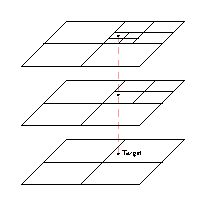
\includegraphics[width=0.6\textwidth]{Figs/Chapter4/map_discretization.pdf}
	\caption{2-Dimensional example of the adopted environment discretization.
			 In this particular case, the presence of a target makes the likelihood level increases in that area, leading to a
			 finer adopted discretization.}
	\label{FIG:SEARCH-SPACE-DISCRETIZATION}
\end{figure}
%%%%%%%%%%
Exact GP inference is expensive due to matrix inversion, whose computational complexity scales with the number of training points as
$\mathcal{O} \lp \nsample^3 \rp$. Moreover, after training, the computation of posterior mean~\eqref{EQ:SEARCH-POST-MEAN} and
variance~\eqref{EQ:SEARCH-POST-VARIANCE} costs $\mathcal{O}\lp \nsample \rp$ and $\mathcal{O} \lp \nsample^2 \rp$ respectively,
per testing point. This makes the application of GP regression in real-time challenging, in particular for large environments.
The common approach to deal with this issue was to divide the environment into regions and train several experts, one for each
region~\cite{kim2013continuous}. This approach was effective, but the complexity problem still persists as long as the number of
observations per region increases. Recently, approaches that leverage on \textit{approximate regression} have shown great success
thanks to their good scaling capabilities~\cite{quinonero2005unifying, wilson2015kernel, gardner2018product}.
To reduce the GP complexity, the adopted approach leverages on the Subset of Regressors (SoR) method~\cite{quinonero2005unifying}
to compute an approximation of the gram matrix $\km$ and the kernel vector $\kv$, jointly with a spatial partitioning and a targeted choice
of the training points. In particular, a set of $\ninducing$ \textit{inducing variables} ($\uu^{1:\ninducing} \in \R^{\ninducing\times3}$)
are arbitrarily selected out of the training points set ($\xx^{1:\nsample}$), then the covariance quantities can be approximated as
\begin{equation}%
	\label{EQ:SEARCH-SOR-APPROX}
	\begin{split}
		\km & \sim \km_{\xx\uu}  \km_{\uu\uu}^{-1} \km_{\uu\xx},\\
		\kv \lp \xx \rp & \sim \km_{\xx\uu} \km_{\uu\uu}^{-1} \kv_{\uu} \lp \xx \rp.
	\end{split}
\end{equation}
Where $\km_{\uu} \in \R^{\ninducing \times \ninducing}$ and $\kv_{\uu} \in \R^{\ninducing}$ are the covariance matrix and vector computed
along the inducing points, while $\km_{\xx\uu} \in \R^{\nsample \times \ninducing}$ is the cross-covariance between $\xx^{1:\nsample}$ and
$\uu^{1:\ninducing}$, with entries
\begin{equation*}
	\km^{i,j}_{\xx\uu} = \kf \lp \xx^i, \uu^j \rp \text{ with } i \in \lps 1, \nsample \rps \text{ and } j \in \lps 1, \ninducing \rps.
\end{equation*}
Plugging~\eqqref{EQ:SEARCH-SOR-APPROX} in~\eqqref{EQ:SEARCH-POST-MEAN} and~\eqqref{EQ:SEARCH-POST-VARIANCE} leads to
\begin{align*}
		\pmu \lp \xx \rp & = \prior \lp \xx \rp + \kv_{\uu} \lp \xx \rp\T \lps \km_{\uu\xx}\km_{\xx\uu} + \nn \km_{\uu\uu} \rps^{-1} \km_{\uu\xx} \cdot \\
						& \hspace{5cm} \cdot \lp \yy^{1:\nsample} - \prior \lp \xx^{1:\nsample} \rp \rp, \\
		\pvar \lp \xx \rp & = \kv_{\uu} \lp \xx \rp\T \lps \km_{\uu\xx}\km_{\xx\uu} + \nn \km_{\uu\uu} \rps^{-1} \kv_{\uu} \lp \xx \rp.
\end{align*}
The SoR approximation method allows to reduce the computation complexity of the training procedure up to $\mathcal{O} \lp \nsample \ninducing^2 \rp$,
while the evaluation complexity of predictive mean and variance is kept constant ($\mathcal{O} \lp \nsample \rp$ and $\mathcal{O} \lp \nsample^2 \rp$,
respectively). The hyper-parameter estimation is carried out by maximizing the log-likelihood function evaluated just on the inducing points
($\log \lp \prob \lp \yy^{1:\ninducing} \mid \uu^{1:\ninducing}; \param \rp \rp$).
In order to further decrease the map computation complexity, we propose a novel methodology to proper select the expert training points.
A good approach should trade-off between process complexity and map precision. To achieve that, the 3-dimensional environment is discretized
with a very coarse resolution, then we let this discretization be flexible in areas where higher precision is required.
The discretization level is then dependent on the local likelihood value: higher is the probability of target existence and finer is the adopted
discretization. In particular, the probability range $[0,1]$ is divided into $q$ intervals, each of which corresponds to a given map resolution.
Note that those intervals are such that a discretization level and the consecutive one differ of a factor equal to $2$.
This leads to a quad-tree space discretization (see~\figref{FIG:SEARCH-SPACE-DISCRETIZATION}). Training points are store in memory only when a
measure of them is retrieved, each new point inherits the current local GP value, then is updated at each new sensor measurement
through~\eqqref{EQ:SEARCH-LOG-LIKELIHOOD}. The adopted hierarchical structure allows to select the inducing variables as those training
points obtained from the coarsest discretization, associated with null probability. Moreover, when a training point gets a promotion to the
upper discretization level, that point is also promoted to inducing variable, while a set of new training points are added to still be
compliant with the associated discretization level.

\subsection{Tree Structure \& Update}%
\label{SEC:SEARCH-TREE-STRUCTURE}
The proposed algorithm works by iteratively growing an RRT, $\tree = \lp \nodes, \edges \rp$, of possible feasible motions,
whose each node $\node_i \in \nodes$ is described by means of six quantities
\begin{equation*}
	\node_i = \left\{ g_i, c_i, \rr_i, \yy_i^{1:\nsample}, \xx_i^{1:\nsample}, \uu_i^{1:\ninducing} \right\},
\end{equation*}
where $g_i = g\lp \node_{i-1}, \node_i \rp$ and $c_i = c\lp \node_{i-1}, \node_i \rp$ are the information gain and the cost,
respectively, associated with the execution of node $\node_i$, i.e. navigate from $\node_{i-1}$ to $\node_i$.
The quantity $\rr_i \in \R^3$ describes the node position, while $\yy_i^{1:\nsample}$, $\xx_i^{1:\nsample}$,
and $\uu_i^{1:\ninducing}$ represent the parameterisation of the likelihood map, at the time of node creation.
As already mentioned, unlike the approach described in~\secref{SEC:EXPLORATION-LARGE-SCALE}, here the adopted tree does not directly
represent a set of possible trajectories, but instead describes a set of feasible paths through the environment.
As a matter of fact, the aforementioned node description does not take into account neither a trajectory parameterisation, nor a
possible execution time. In this sense, two nodes $\node_{i-1}$ and $\node_i$ are connected by an edge $\edge_{i-1}$ if the straight path
connecting $\rr_{i-1}$ and $\rr_i$ is collision-free, no other continuity constraints are required.
Although the nodes present a slight different structure, the aim of this tree is the same of the one build in~\secref{SEC:EXPLORATION-TREE-STRUCTURE}.
Basically, the goal is to compute sub-optimal paths that maximise a given utility function $\loss \lp \RR \lp \node_i \rp \rp$, with
the latter that combines gains and costs of all nodes in $\RR \lp \node_i \rp$. It results that the final agent behavior strongly depends
on the chosen functions $g \lp \node_{i-1}, \node_i \rp$, $c \lp \node_{i-1}, \node_i \rp$ and $\loss \lp \RR \lp \node_i \rp \rp$.
Unlike general planners, who exploit RRT structures to plan flyable trajectories, in this case the tree expansion logic
must be designed around the aforementioned loss functions, with particular attention to the gain $g \lp \node_{i-1}, \node_i \rp$.
Tailoring the algorithm behavior on $g$ allows for keeping the exploration task consistent during the motion, and avoids cases
in which the agent gets stuck in little areas, without exploring the overall environment. This is particularly true when the
chosen utility function presents many local minima, which are difficult to escape.
In this respect, we formulate a new information gain index that takes into account the amount of improvement, in the current
likelihood map, brought by the execution of the considered node. In particular, consider two nodes $N_{i-1}$ and $N_i$,
with their respective map parameterisation $\pmu_{i-1} \lp \yy_{i-1}^{1:\nsample}, \xx_{i-1}^{1:\nsample}, \uu_{i-1}^{1:\ninducing}, \xx \rp$
and $\pmu_{i} \lp \yy_{i}^{1:\nsample}, \xx_{i}^{1:\nsample}, \uu_{i}^{1:\ninducing}, \xx \rp$, the gain associated with the
node $\node_i$ can be evaluated as
\begin{equation*}
	g_i \lp \node_i, \node_{i-1} \rp = \int_{\E} \frac{\exp \lp \pmu_{i-i} \lp \cdot, \xx \rp \rp}{1 + \exp \lp \pmu_{i-i} \lp \cdot, \xx \rp \rp} -
								  	   \frac{\exp \lp \pmu_i \lp \cdot, \xx \rp \rp}{1 + \exp \lp \pmu_i \lp \cdot, \xx \rp \rp} d\xx,
\end{equation*}
where the quantities $\yy_{i}^{1:\nsample}$, $\xx_{i}^{1:\nsample}$, and $\uu_{i}^{1:\ninducing}$ are computed out of the corresponding
values of the $\node_{i-1}$ node via~\eqqref{EQ:SEARCH-LOG-LIKELIHOOD}, along the path connecting $\rr_{i-1}$ to $\rr_i$.
Note that, unlike previous works in this field~\cite{popovic2020informative, schmid2020efficient}, here the information gain is not
a function of the node end-position only, thus allows us to consider also frustrum overlap between consecutive poses and the amount of
information gained while moving from $\node_{i-1}$ to $\node_i$.
On the other hand, the node execution cost is fixed as the intra-node Euclidean distance $c_i \lp \node_i, \node_{i-1} \rp = \norm{\rr_{i-1} - \rr_i}$,
while the total utility function as been designed following the same idea of efficiency stated in~\secref{SEC:EXPLORATION-COST-FUNCTIONS}
\begin{equation*}
	\loss \lp \RR(\node_i) \rp = \frac{\sum_{\node_l \in \RR \lp \node_i \rp} g_l}{\sum_{\node_l \in \RR \lp \node_i \rp} c_l}.
\end{equation*}
With these notion at hand, we can now proceed to the design of the core of the algorithm. The chosen tree updating procedure is
as simple as it is effective, and it is designed to cope with the multi-modal nature of the chosen utility function, as well as
the possibility to inject prior notions about the obstacles occupancy. The tree, initially composed of just one root node, is
iteratively expanded via random sampling of the next node position $\rr_i$. In particular, we constrain the sample points to lie
inside a circular crown of radii $R_{\text{min}}$ and $R_{\text{max}}$, centered on the current best node ($\node_{\text{best}}$),
namely the one among all tree nodes that maximise the utility function $\loss \lp \cdot \rp$. In order to escape from local minima
and let the tree grow in all directions, the best node is reevaluated each $n_{\text{sample}}$ samples, ensuring that every expanded
node presents exactly $n_{\text{sample}}$ childs. This choice, jointly with the circular crown constraint, allows the algorithm to
expand the tree without getting stuck in little areas, with many local minima.
Each sampled viewpoint is retained only if it belongs to a known and free part of the environment and, at the same time, the line
connecting it with the respective father is far enough from the mapped obstacles. The tree expansion continues until
the number of sampled nodes goes beyond a given threshold $n_{\text{max}}$, then the path connecting the root node to the best one
is extracted and completely executed. It may happen that, the autonomous robot is not able to complete the commissioned path due 
to unexpected obstructions, in this case the algorithm keeps track of the executed nodes and reinitialize the tree with the 
final executed node as root.

\subsection{B-Spline Trajectory Optimisation}%
\label{SEC:SEARCH-TRAJECTORY-OPTIMISATION}
As already pointed out in previous sections, the built tree does not directly represent flyable trajectories, but just feasible paths
through the environment's obstacles. For the purpose of control, a timing law is essential to ensure the dynamic feasibility of the resulting
reference. In the specific case of a quadcopter, such a reference can be computed just in terms of heading angle $\yaw$ and space position
$\rr = \lps x, y, z \rps \in \R^3$, following the concept of differential flatness~\cite{mellinger2011minimum}. The latter property can
be used only if the heading trajectory is guarante to be at least a class $\CC^1$ function, while $\rr$ must be at least class $\CC^3$.
Contrary to the solution presented in~\secref{SEC:EXPLORATION-LARGE-SCALE}, here we enforce the use of B-splines as time parameterisation
tool for the planned collision-free path. B-splines are a generalization of B\acuteacc ezier curves which allows for a more compact
representation, especially when dealing with long trajectory segments. Unlike B\acuteacc ezier curves, B-splines are defined by a
set of control points $\CP = \lps \bs{\cpoint}_0, \dots, \bs{\cpoint}_{\cpnumber} \rps$, and a set of time knots
$\bs{\splinevar} = \lps \splinevar_0, \dots, \splinevar_{\cpnumber + \order + 1} \rps$, as
\begin{equation*}
	\bs{\spline} \lp \splinevar \rp = \sum_{i=0}^\cpnumber \basis_i^\order \lp \splinevar \rp \bs{\cpoint}_i,
\end{equation*}
with $\order$ order of the spline and $\basis_i^\order$ basis functions, recursively computed via the De-Boor formula~\cite{de1978practical}.
B-splines and B\acuteacc ezier curves share several properties, among all, the most important ones at the time being, are the
(a) convex hull containment and (b) closure with respect to differentiation. These two properties allow to easily formulate
a constrained quadratic programming problem and solve it for the final trajectory control points. A deeper analysis of B-spline properties and
their evaluation is reported in~\secref{SEC:SPLINES-APPENDIX}. In the specific case of patrolling, since we are using a downward-facing camera, the
heading trajectory loses importance, thus we consider it as a constant reference in time, and focus only on solving the optimisation problem
for the $x$, $y$, and $z$ components. Suppose to discretize the node sequence $\RR \lp \node_{\text{best}} \rp$ with a given resolution $\Delta_{\rr}$,
leading to a sequence of waypoints, $\rr_0, \cdots, \rr_{\cpnumber}$, moreover let $\order = 7$ and fix the knot vector as
\begin{equation*}
	\bs{\splinevar} =
	\begin{bmatrix}
		0_{0:7}, & \Delta_{\splinevar}, & 2\Delta_{\splinevar}, & \dots, & (\cpnumber-\order)\Delta_{\splinevar}, & T_{0:7}
	\end{bmatrix},
\end{equation*}
with $T = \sum_{i=0}^{\cpnumber-1} \norm{\rr_i - \rr_{i+1}}/v_{\text{max}}$ and $\Delta_{\splinevar} = T/(\cpnumber - \order + 1)$.
Then, the problem of feasible trajectory generation can be solved via the constrained quadratic programming
\begin{equation}%
	\label{EQ:SEARCH-OPTIMISATION-PROBLEM}
	\begin{split}
	\min_{\bs{\cpoint}_{0}, \dots, \bs{\cpoint}_{\cpnumber}} &
				\lambda_1 \int_0^{T} \norm{\frac{d^3 \bs{\spline} \lp \splinevar \rp}{d \splinevar^3}}^2 d \splinevar
				+ \lambda_2 \sum_{i=0}^{\cpnumber} \norm{\bs{\cpoint}_i - \rr_i}^2, \\
	\text{sub.to.} \hspace{0.3cm} &
				\bs{\cpoint}_i' \le v_{\text{max}} \hspace{0.3cm} \forall i = 0, \dots, \cpnumber-1, \\
				& \bs{\cpoint}_i'' \le a_{\text{max}} \hspace{0.3cm} \forall i = 0, \dots, \cpnumber-2, \\
				& \bs{\cpoint}_0 = \rr_0, \hspace{0.3cm} \bs{\cpoint}_{\cpnumber} = \rr_{\cpnumber}, \\
				& \bs{\cpoint}_0' = v_{\text{init}}, \hspace{0.3cm} \bs{\cpoint}_0'' = a_{\text{init}},
	\end{split}
\end{equation}
with $\lambda_{1,2} \in \R$ tuning parameters and $v_{\text{max}}$, $a_{\text{max}}$, $v_{\text{init}}$, and $a_{\text{init}}$ provided as
inputs. The aforementioned optimisation problem, framed in the context of quadcopter control, tries to compute minimal effort trajectories that
propagate in time close to the sampled waypoints. The B-spline properties are used here to constrain the dynamical quantities to strictly
remain inside the imposed structural limits and to shape the curve along the selected viewpoints.
Note that no final velocity nor acceleration constraints have been imposed, letting the algorithm select the optimal ones on its own.
This choice is motivated by the discussion carried out in~\secref{SEC:EXPLORATION-LARGE-SCALE}, where emerges that constraining the robot
to stop at each exploration step may degrade the algorithm performance.
As in the case of B\acuteacc ezier curves (see~\secref{SEC:EXPLORATION-COST-FUNCTIONS}), the loss function in
problem~\eqref{EQ:SEARCH-OPTIMISATION-PROBLEM} can be fully decomposed along the tree axis, yielding
\begin{equation*}
	\begin{split}
	\min_{\bs{\cpoint}_{0}, \dots, \bs{\cpoint}_{\cpnumber}} &
				\sum_{j}^{x,y,z} \lps \lambda_1 \int_0^{T} \lp \frac{d^3 \bs{\spline}_j \lp \splinevar \rp}{d \splinevar^3} \rp^2 d \splinevar
				+ \lambda_2 \sum_{i=0}^{\cpnumber} \lp \bs{\cpoint}_{j,i} - \rr_{j,i} \rp^2 \rps, \\
	\text{sub.to.} \hspace{0.3cm} &
				\text{Same of problem~\eqref{EQ:SEARCH-OPTIMISATION-PROBLEM}}.
	\end{split}
\end{equation*}
% For an eventually interested reader, a deeper analysis about this optimisation technique, how it can be implemented,
% extended and adapted to other use cases is reported in~\secref{SEC:TRAJECTORY-GENERATION}.

\subsection{Experimetal Results \& Future Directions}%
\label{SEC:SEARCH-EXPERIMENTAL-RESULTS}
%%%%%%%%%%
\begin{figure}[!t]
	\begin{center}
		\begin{minipage}{.4\linewidth}
			\centering
			\subfloat[]{%
				\label{FIG:SEARCH-RESULTS-MAP-A}%
				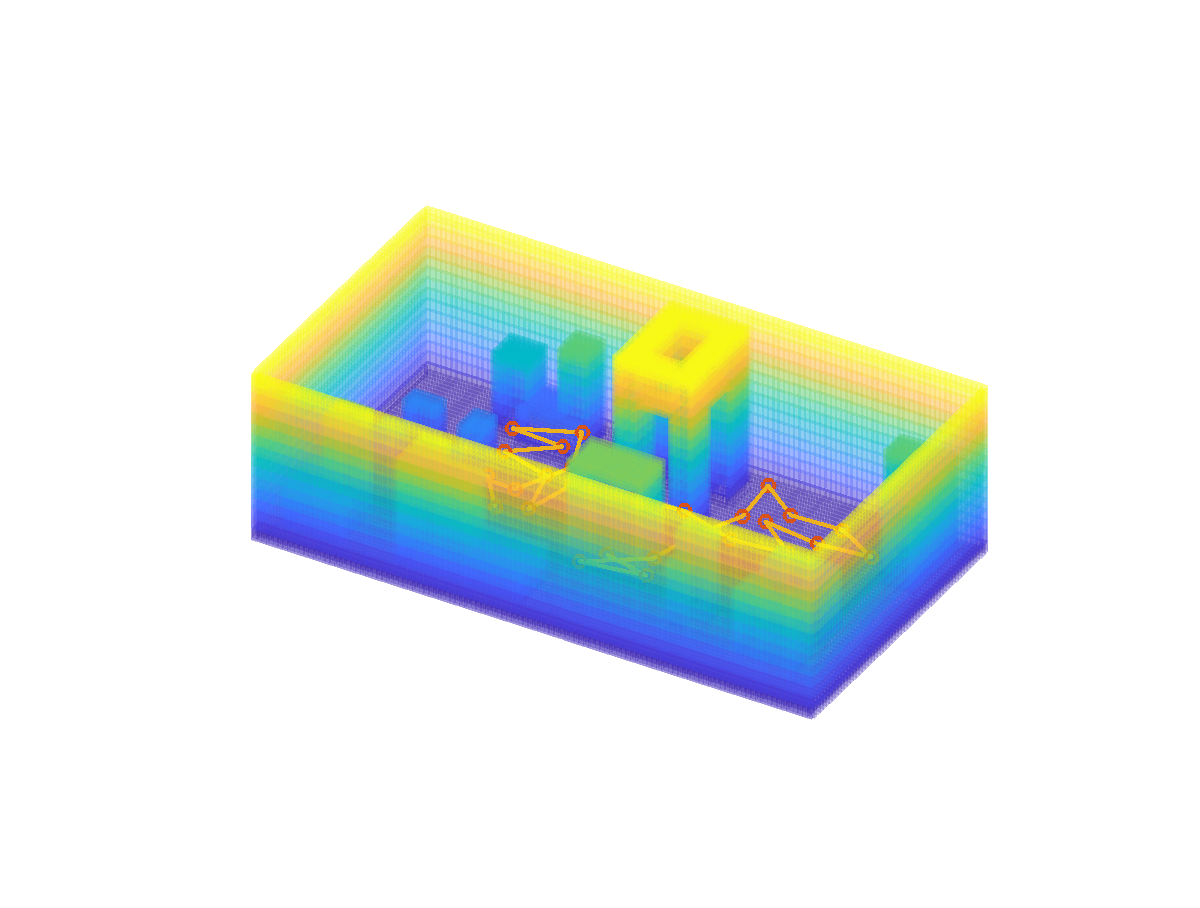
\includegraphics[trim={3.5cm 1.5cm 3cm 2.2cm}, clip = true, width = 1\textwidth]{Figs/Chapter4/search_map_1steps.eps}}
		\end{minipage}
		\begin{minipage}{.4\linewidth}
			\centering
			\subfloat[]{%
				\label{FIG:SEARCH-RESULTS-MAP-B}%
				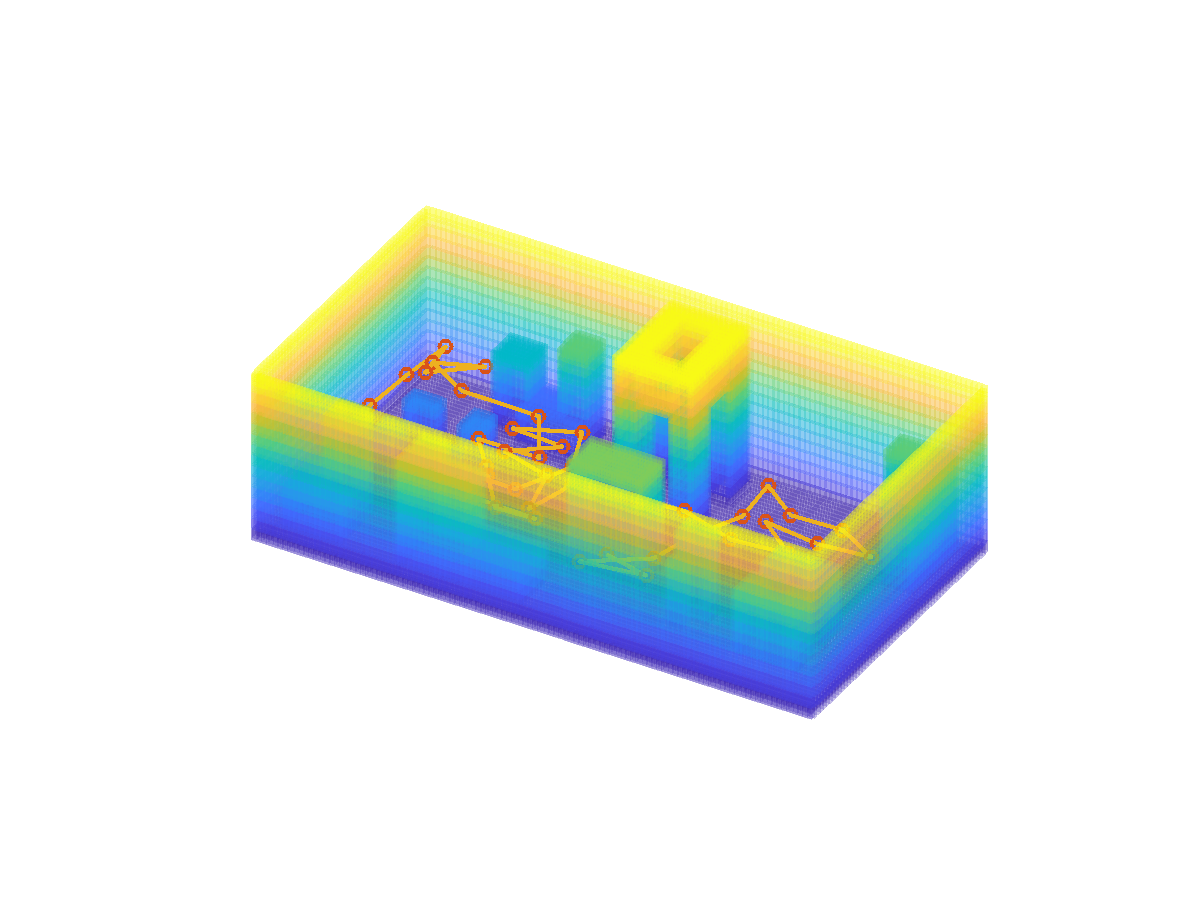
\includegraphics[trim={3.5cm 1.5cm 3cm 2.2cm}, clip = true, width = 1\textwidth]{Figs/Chapter4/search_map_2steps.eps}}
		\end{minipage}
		\begin{minipage}{.4\linewidth}
			\centering
			\subfloat[]{%
				\label{FIG:SEARCH-RESULTS-MAP-C}%
				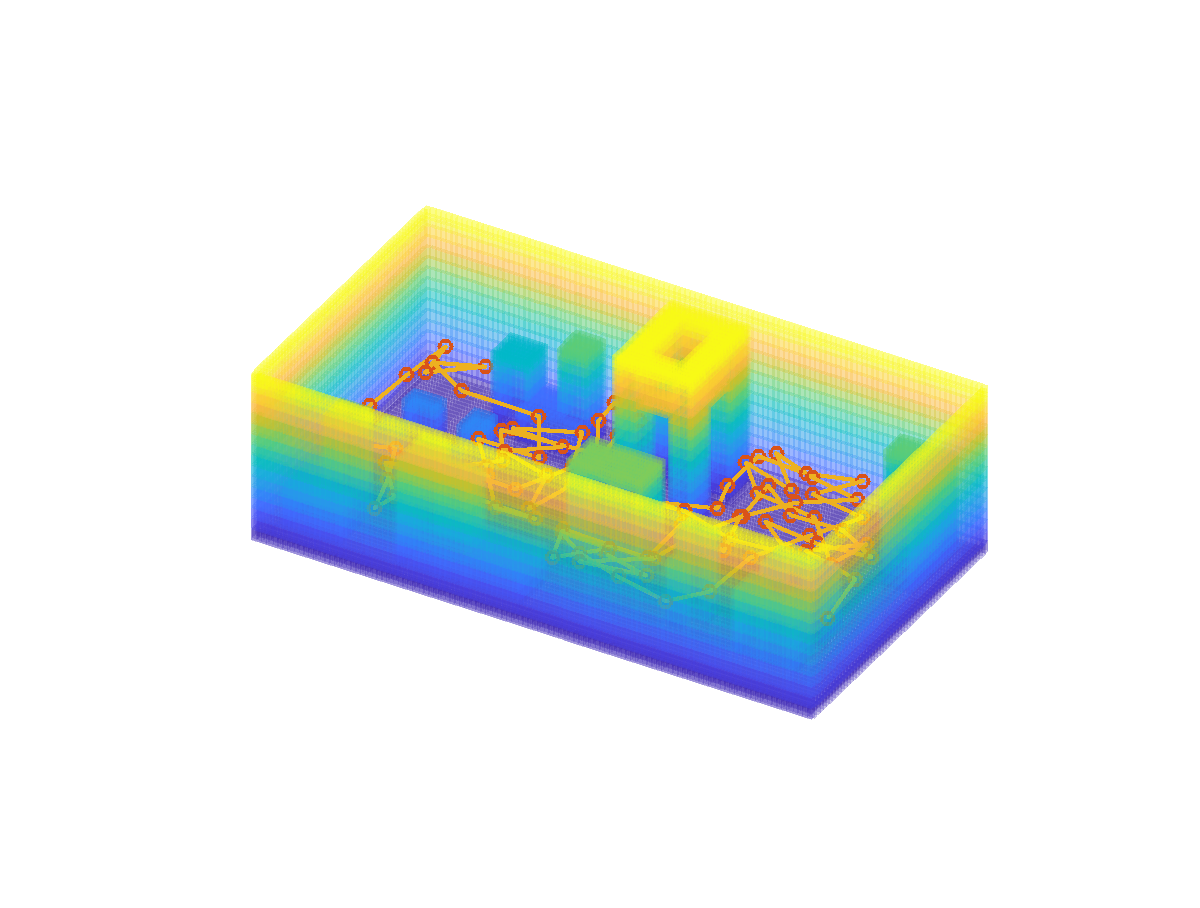
\includegraphics[trim={3.5cm 1.5cm 3cm 2.2cm}, clip = true, width = 1\textwidth]{Figs/Chapter4/search_map_5steps.eps}}
		\end{minipage}
	\end{center}
	\caption{Results of the proposed search algorithm. The figure depicts the simulated environment along with the built
	tree of possible viewpoints. Red circles represent the tree nodes, while the yellow connecting lines its edges.
	In the image, in order, (a) exploration state after only one step, (b) after two steps, and (c) after five steps.
	Note how the tree grows toward previously unexplored areas.}\label{FIG:SEARCH-RESULTS-MAP}
\end{figure}
%%%%%%%%%%
The proposed approach has been tested on a synthetic urban canyon scenario, similar to the one proposed during the Leonardo drone
contest during the third year (see~\secref{SEC:DRONE-CONTEST}). In this scenario, the $10 \times 20 \times 3$ meters map was already completely
known in advance and the flying agent was required to find as fast as possible a single moving unmanned ground robot. Thanks to these experiment
settings the explorer was initialized with a prior guess of probability distribution that equalizes to zero near and over the known
obstacles. The obtained results are reported in~\figref{FIG:SEARCH-RESULTS-MAP},~\ref{FIG:SEARCH-RESULTS-TRAJECTORY}, and~\ref{FIG:SEARCH-RESULTS-COST}.
In particular,~\figref{FIG:SEARCH-RESULTS-MAP} depicts the built tree, where red circles represent nodes and the yellow connecting lines the
tree edges, along with a discrete representation of the environment map. Overlapping~\figref{FIG:SEARCH-RESULTS-MAP} with~\figref{FIG:SEARCH-RESULTS-TRAJECTORY}
the blue continuous line represents the final trajectory followed by the drone during the exploration task. Finally,~\figref{FIG:SEARCH-RESULTS-COST}
reports the used probability map. In all the figures, in order, has been depicted the exploration state after one, two, and five steps.
Note how the agent tends to explore quickly previously unseen areas, while the probability increases over time in not visited areas and
decreases a lot after one agent visit. The proposed solution has been successfully employed during the Leonardo challenge, where
the drone was able to find out the ground agent in almost a couple of minutes, with a maximum velocity of $0.5m/s$ and starting always
from random initial positions. The algorithm was able to run completely real-time with only onboard computation and sensing capabilities.
For a complete list of the used parameters, please refer to~\tabref{TAB:SEARCH-PARAMETERS}.

In this section, we proposed a novel solution to the exploration problem in the setting where target search is the only final goal.
This approach is in contrast with the one described in~\secref{SEC:EXPLORATION-LARGE-SCALE} under different aspects, first it plans paths
instead of directly flyable trajectories, this approach may lead to degraded performances in all those cases in which the environment
is not a priori known, constraining the agent to perform several stops before starting a new exploration step. On the other hand, the latter
solution allows for continuous mapping of the target probability, which is constantly kept updated during the tree expansion.
Future research directions in this field may aim to fill the gap between these two solutions and try to solve both the problem of
environment exploration and target finding concurrently. At the same time, we wish to import the local-global paradigm even in this
class of problems, which currently is not considered yet.
%%%%%%%%%%
\begin{figure}[!t]
	\begin{center}
		\begin{minipage}{.4\linewidth}
			\centering
			\subfloat[]{%
				\label{FIG:SEARCH-RESULTS-TRAJECTORY-A}%
				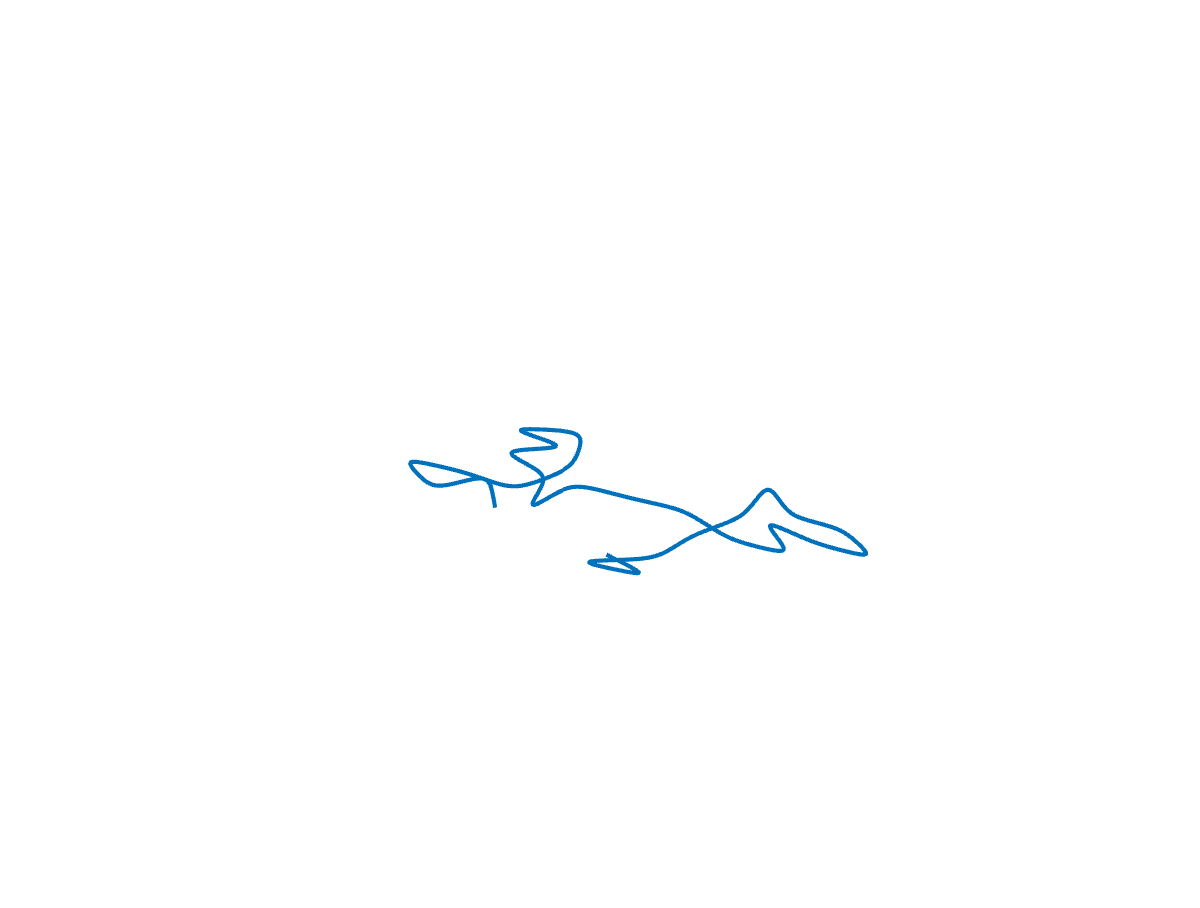
\includegraphics[trim={3.5cm 3cm 3cm 4cm}, clip = true, width = 1\textwidth]{Figs/Chapter4/search_traj_1steps.eps}}
		\end{minipage}
		\begin{minipage}{.4\linewidth}
			\centering
			\subfloat[]{%
				\label{FIG:SEARCH-RESULTS-TRAJECTORY-B}%
				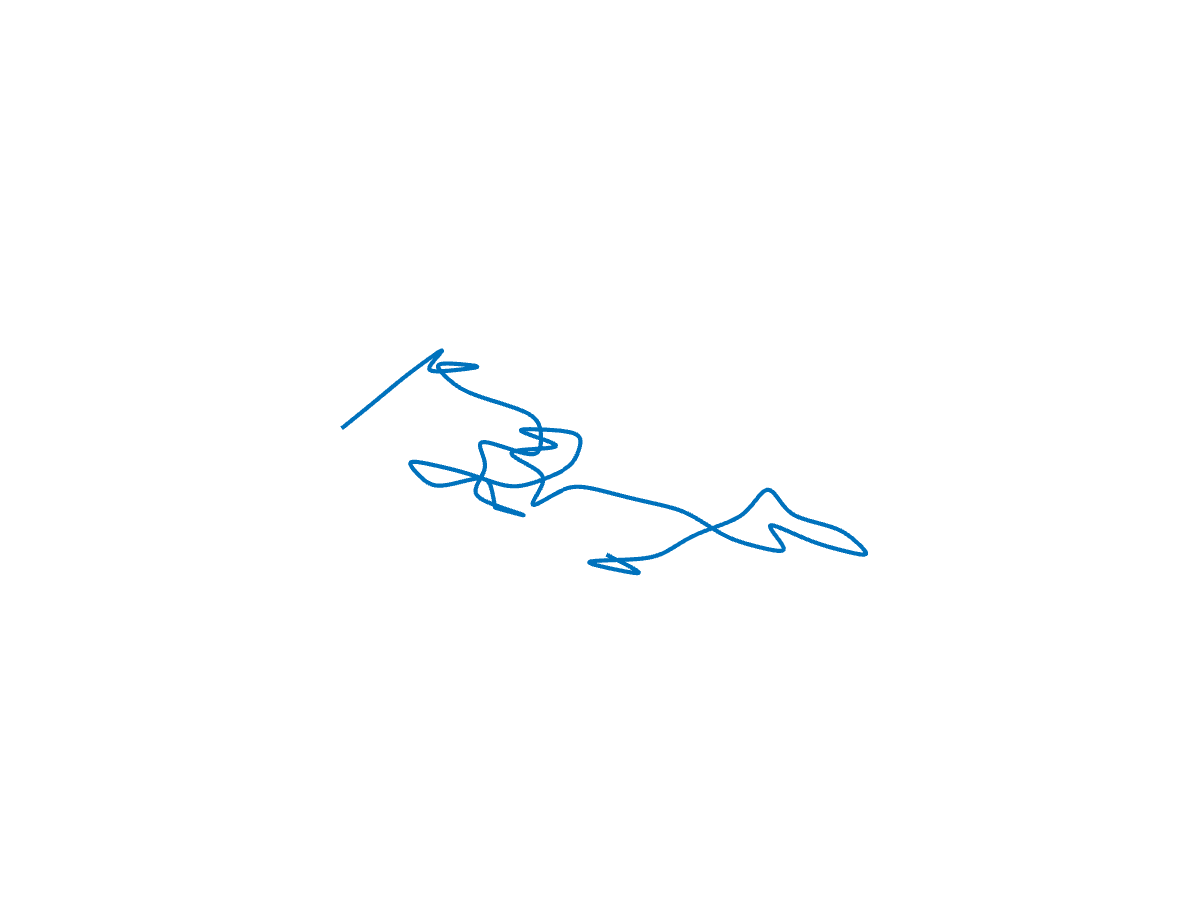
\includegraphics[trim={3.5cm 3cm 3cm 4cm}, clip = true, width = 1\textwidth]{Figs/Chapter4/search_traj_2steps.eps}}
		\end{minipage}
		\begin{minipage}{.4\linewidth}
			\centering
			\subfloat[]{%
				\label{FIG:SEARCH-RESULTS-TRAJECTORY-C}%
				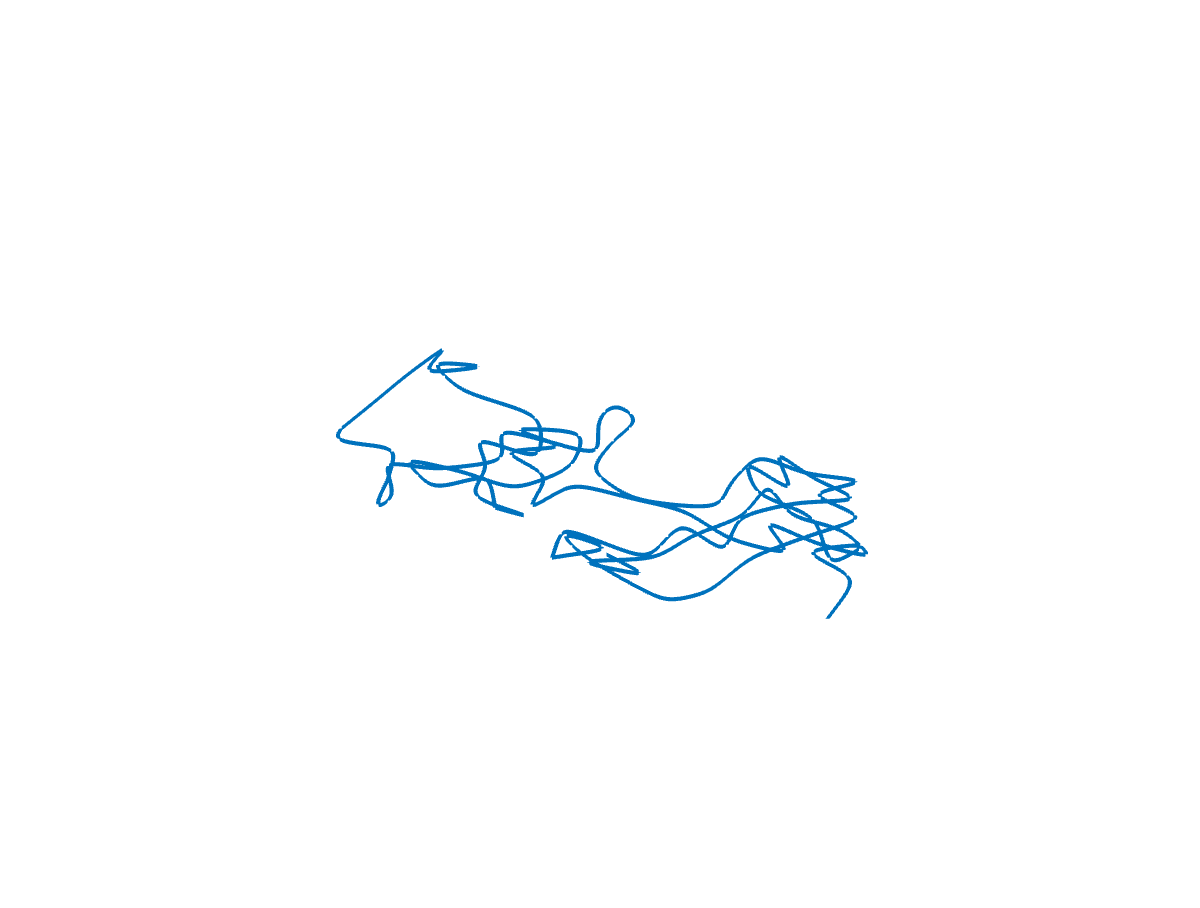
\includegraphics[trim={3.5cm 3cm 3cm 4cm}, clip = true, width = 1\textwidth]{Figs/Chapter4/search_traj_5steps.eps}}
		\end{minipage}
	\end{center}
	\caption{Results of the proposed search algorithm. The figure depicts the planned reference trajectory after (a) one exploration step,
	(b) two exploration steps, and (c) five exploration steps. The reported trajectory is built on top of the viewpoints tree reported
	in~\figref{FIG:SEARCH-RESULTS-MAP}.}\label{FIG:SEARCH-RESULTS-TRAJECTORY}
\end{figure}
%%%%%%%%%%
%%%%%%%%%%
\begin{figure}[!t]
	\begin{center}
		\begin{minipage}{.4\linewidth}
			\centering
			\subfloat[]{%
				\label{FIG:SEARCH-RESULTS-COST-A}%
				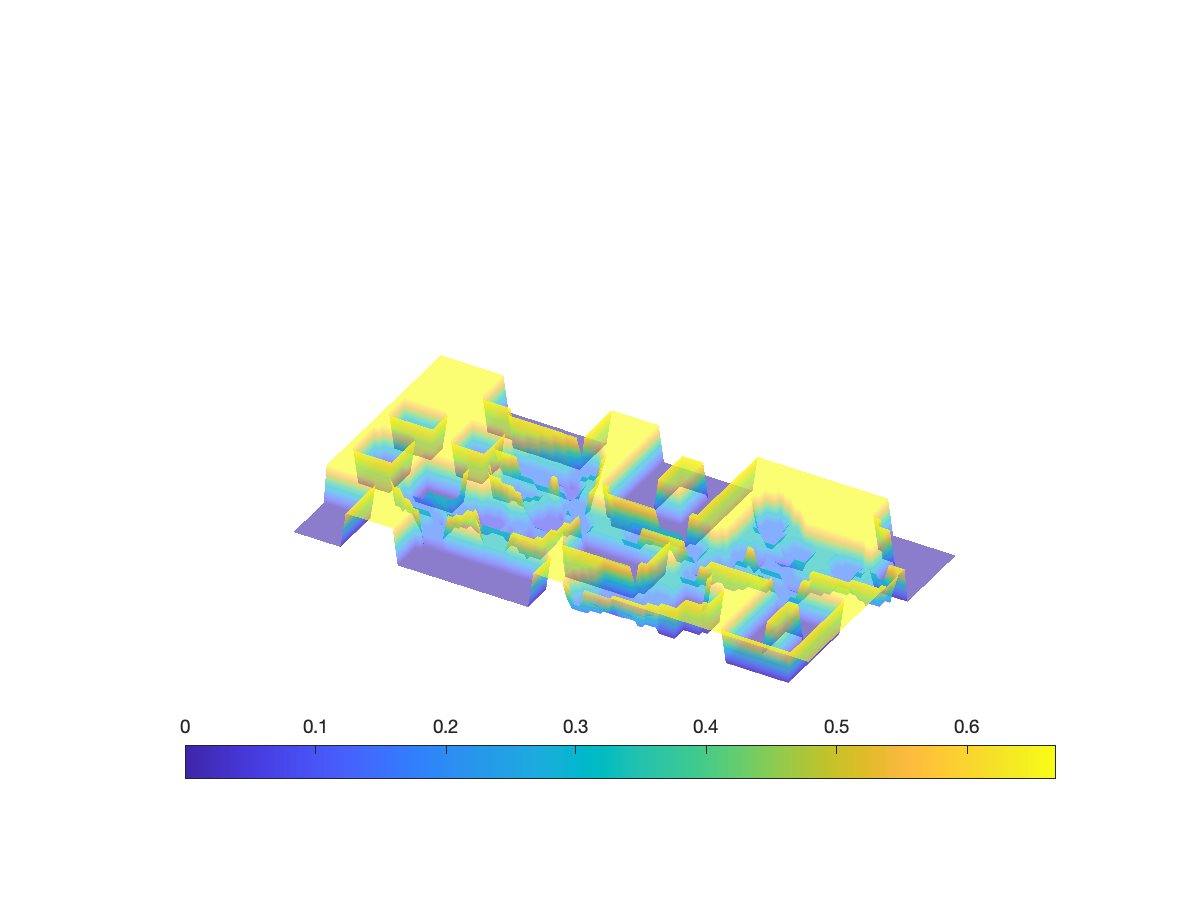
\includegraphics[trim={3.5cm 1.5cm 2cm 4cm}, clip = true, width = 1\textwidth]{Figs/Chapter4/search_cost_1steps.eps}}
		\end{minipage}
		\begin{minipage}{.4\linewidth}
			\centering
			\subfloat[]{%
				\label{FIG:SEARCH-RESULTS-COST-B}%
				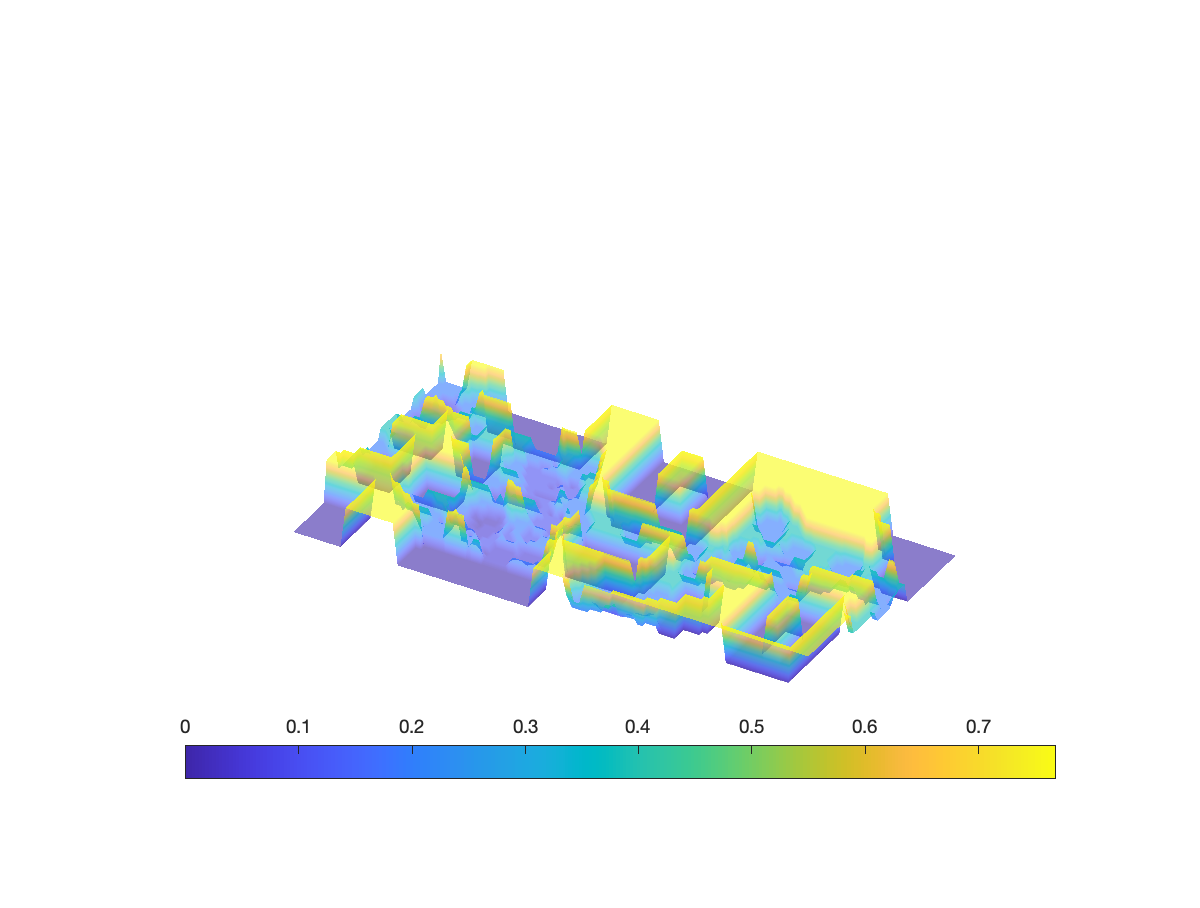
\includegraphics[trim={3.5cm 1.5cm 2cm 4cm}, clip = true, width = 1\textwidth]{Figs/Chapter4/search_cost_2steps.eps}}
		\end{minipage}
		\begin{minipage}{.4\linewidth}
			\centering
			\subfloat[]{%
				\label{FIG:SEARCH-RESULTS-COST-C}%
				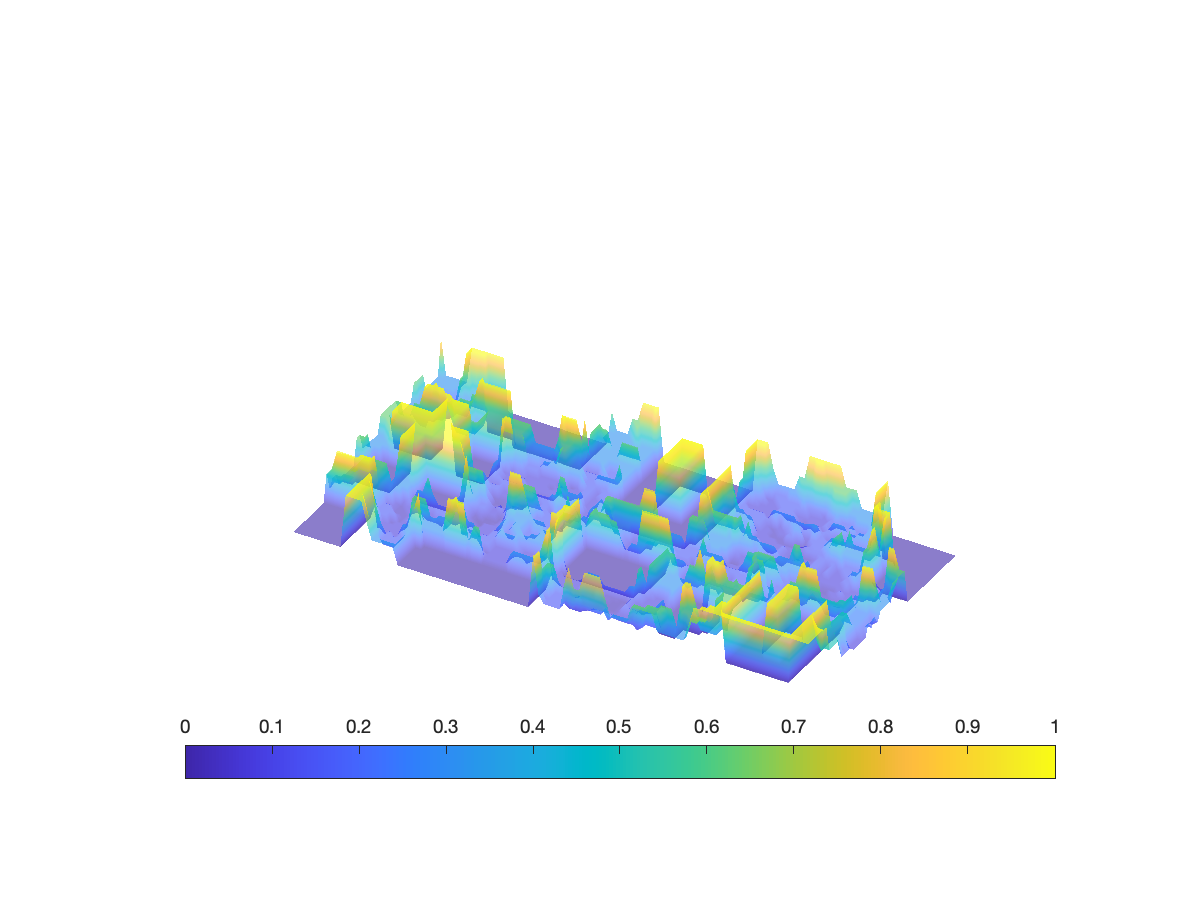
\includegraphics[trim={3.5cm 1.5cm 2cm 4cm}, clip = true, width = 1\textwidth]{Figs/Chapter4/search_cost_5steps.eps}}
		\end{minipage}
	\end{center}
	\caption{Results of the proposed search algorithm. The figure depicts the costmap state during the searching task after
	(a) one exploration step, (b) two exploration steps, and (c) five exploration steps.
	The reported costmap is used to build the tree of possible viewpoints reported in~\figref{FIG:SEARCH-RESULTS-MAP}.
	Note how the cost decreases a lot after each agent visit, how it increases in time in not visited areas, and how the cost
	is almost zero on obstacle cells. The latter property can be easily integrated into the algorithm thanks to its flexibility to
	apriori knowledge about probability distributions.}\label{FIG:SEARCH-RESULTS-COST}
\end{figure}
%%%%%%%%%%
%%%%%%%%%
{
\renewcommand{\arraystretch}{1.35}
\begin{table}[b!]
    \centering
    \begin{tabular}{||c|c||c|c||}
        \hline
        \hline
        $n_{\text{max}}$ & $1500$ & $n_{\text{sample}}$ & $60$ \\
        \hline
        $R_{\text{min}}$ & $0.5m$ & $R_{\text{max}}$ & $4.0m$ \\
        \hline
        $v_{\text{max}}$ & $0.5m/s$ & $a_{\text{max}}$ & $0.5 m/s^2$ \\
        \hline
        $p^{\text{inc}}$ & $1.01$ & $p_{\text{max}}^{\text{dec}}$ & $0.5$ \\
		\hline
		$W$ & $\lps 5, 0; 0, 5 \rps$ & $c$ & $0.0$ \\
		\hline
		$\lambda_1$ & $1.0$ & $\lambda_2$ & $10.0$ \\
        \hline
        \hline
    \end{tabular}
    \caption{Parameters used to test the object search algorithm.}%
	\label{TAB:SEARCH-PARAMETERS}
\end{table}}
%%%%%%%%%

%----------------------------------------------------------------------------------------
\section{Contributions}
This chapter is devoted to reviewing two original approaches to the problem of rapid exploration in two different contexts.
In the first stage, the focus is on the robot's capabilities and the employed algorithm is meant to carry out the exploration task
as fast as possible pushing the drone on the boundaries of its dynamical limits. While in the second stage, the focus is on the
exploration for target search. In this second case, the proposed solution mixes a continuous mapping paradigm with the random
nature of RRTs. It results in two approaches able to sequentially build high informative trajectories, or paths, in unknown, partially
known or completely known environments. In both cases, Gaussian processes have been used to fast infer the node's information gain, and
both approaches have been validated with real scenario tests. As previously mentioned, we propose, as future work to bridge the gap
between these two solutions and try to solve both the problems of environment exploration and target searching concurrently, by
planning directly sub-optimal and feasible trajectories.
We believe that the introduction of these solutions opens a new research frontier able to cope with the gap between the learning theory,
from supervised to unsupervised techniques, and the robotic world, where the limited computational power does not allows for
online network training or big data processing.

%------------------------------------------------